% The TFG book: purpose, data, methods, analyses, sources, and how to build on them.
% Build (from this folder): pdflatex main.tex  (run twice for the table of contents)
\documentclass[11pt,a4paper,openany]{book}
\usepackage[utf8]{inputenc}
\usepackage[T1]{fontenc}
\usepackage{lmodern}
\usepackage{amsmath,amssymb}
\usepackage[margin=2.5cm]{geometry}
\usepackage{booktabs,tabularx,longtable,array}
\usepackage{enumitem}
\usepackage{xcolor}
\usepackage{graphicx}
\usepackage{listings}
\usepackage[most]{tcolorbox}
\usepackage[hidelinks]{hyperref}
\usepackage{microtype}
\usepackage{url}
\urlstyle{tt}

\graphicspath{{../../experiments/01-reply-opposition-lifetime/results/}}

\setlist{itemsep=2pt,topsep=4pt}
\setlength{\parindent}{0pt}
\setlength{\parskip}{6pt}
\renewcommand{\arraystretch}{1.15}
\newcolumntype{Y}{>{\raggedright\arraybackslash}X}

\lstset{basicstyle=\ttfamily\footnotesize,breaklines=true,frame=single,
  backgroundcolor=\color{black!3},numbers=none,columns=fullflexible,keepspaces=true}

\newcommand{\file}[1]{\path{#1}}
\newcommand{\todo}[1]{\textcolor{red!70!black}{[#1]}}
\newcommand{\src}[1]{\textcolor{blue!50!black}{[#1]}}

% Boxes used throughout
\newtcolorbox{idea}[1][]{colback=blue!4,colframe=blue!50!black,title=In one sentence,fonttitle=\bfseries\small,sharp corners,boxrule=0.5pt,#1}
\newtcolorbox{pitfall}[1][]{colback=red!4,colframe=red!60!black,title=Pitfall,fonttitle=\bfseries\small,sharp corners,boxrule=0.5pt,#1}
\newtcolorbox{tryit}[1][]{colback=green!4,colframe=green!40!black,title=Try it yourself,fonttitle=\bfseries\small,sharp corners,boxrule=0.5pt,#1}
\newtcolorbox{readbox}[1][]{colback=black!4,colframe=black!50,title=How to read this figure,fonttitle=\bfseries\small,sharp corners,boxrule=0.5pt,#1}

\title{\textbf{Who replies to whom, and how long do they stay?}\\[6pt]
\Large A reader's book on my TFG:\\ replies, vote-based opposition and user lifetime on DerStandard.at}
\author{Working book, state of 2026-11-03}
\date{}

\begin{document}
\frontmatter
\maketitle
\tableofcontents
\mainmatter

\chapter*{Preface: how to read this book}
\addcontentsline{toc}{chapter}{Preface: how to read this book}

\textbf{Written for:} you, the author of the TFG, who has seen the results but has not yet had time to understand every method and wants to be able to extend the work alone.

\section*{What this book is}
The repository holds the code, the notes and the results of the first experiment of the TFG. Those files are written for someone who already knows the project. This book is written for someone who is \emph{learning} the project. It tells the story in order, explains each idea with small numbers you can check by hand, shows where every piece lives in the code, says honestly what is weak, and ends with recipes for doing your own analyses.

It replaces the two earlier guides in this folder (\file{tfg-guide.pdf}, a map, and \file{methods-study-guide.pdf}, a methods primer). They are kept; their material is reused here and expanded.

\section*{What this book is not}
It is not a statistics textbook. When a method needs more depth than a page or two, the text says so and points to a source in Chapter~\ref{ch:sources}, with a note on which chapter or section to read and how long it takes.

\section*{Three ways to read it}
\begin{description}
  \item[Cover to cover (about 6--8 hours).] The order is the logical order: why $\to$ data $\to$ tools $\to$ methods $\to$ code $\to$ results $\to$ doubts $\to$ sources $\to$ your own work.
  \item[Before a meeting (about 1 hour).] Chapter~\ref{ch:purpose}, the summary boxes at the start of each method in Chapter~\ref{ch:methods}, the table in Section~\ref{sec:headline}, and Chapter~\ref{ch:critique}.
  \item[To build something new (about 2 hours).] Chapter~\ref{ch:pipeline} (how the pieces connect), then Chapter~\ref{ch:building}. Come back to Chapter~\ref{ch:methods} for any method you reuse.
\end{description}

\section*{Boxes and conventions}
\begin{idea}
A blue box gives the idea of a section in one sentence. If you only remember one thing, remember this.
\end{idea}
\begin{pitfall}
A red box names a typical misreading or a typical mistake.
\end{pitfall}
\begin{tryit}
A green box asks you to do something small: compute by hand, run a snippet, change a number. Learning happens here. Answers to the exercises are in Appendix~\ref{app:exercises}.
\end{tryit}

File names are written like \file{04\_h1\_comment\_level.py}. Paths are relative to the \file{tfg/} folder. Square brackets such as \src{Mantel \& Haenszel 1959} refer to Chapter~\ref{ch:sources}.

\section*{Status of the claims}
Parts of the first analysis were done with an AI assistant (see \file{notes/method/AI-USE.md}). Every decision in the repository is tagged \emph{me}, \emph{AI, reviewed} or \emph{AI, not yet reviewed}. A goal of this book is that none of the decisions remains in the last category because you could not explain it. Chapter~\ref{ch:critique} lists what a line-by-line code review found; none of it changes a headline number, but several points limit what you may claim.

\section*{A note on how much is settled}
The headline results are numbers produced by code that was reviewed. The \emph{interpretation} of some of them is still open: for instance, whether the ``long-lived users'' result describes a trait of the users or just a property of how the group was defined (Section~\ref{sec:longlived}). Where interpretation is open, the book says so.

\chapter{Purpose and context}\label{ch:purpose}

\section{The project in one page}
The TFG is supervised by Andreas Kaltenbrunner (UPF) and uses the \emph{DerStandard} dataset built by his group: ten years (2013--2022) of threaded comments and up/down votes from the forum of an Austrian newspaper, DerStandard.at \src{Fraxanet et al.\ 2026}. In the first meeting (2026-09-30) the task was set as:

\begin{quote}
\emph{Analyse who replies to whom, whether their positions are opposed, and complement it with an analysis of users' lifetime.}
\end{quote}

Three words in that sentence need unpacking.
\begin{description}
  \item[Replies.] A comment can answer another comment. That creates a directed edge from the replier $A$ to the author $B$ of the comment answered. The dataset gives the parent of each reply, so the reply network is observed, not guessed.
  \item[Opposed positions.] The dataset has \emph{no comment text}, so we cannot read what people say. What we do have is votes: who gave a thumbs-up or thumbs-down to which comment. We use votes as a \emph{proxy for stance}: if $A$ keeps downvoting $B$'s comments, $A$ is probably against $B$. This is the central modelling choice of the thesis, and you should be ready to defend it and to name its limits (Chapter~\ref{ch:critique}).
  \item[Lifetime.] For each user, the time between first and last activity. Users who leave are interesting for community health; the question is whether what happens to a newcomer in the first weeks (being downvoted, receiving hostile replies) is related to how long they stay.
\end{description}

\begin{idea}
The thesis asks three linked questions: do people reply to those they vote against (stance), is that pattern stronger than chance (a null model), and is early exposure to it related to leaving sooner (survival)?
\end{idea}

\section{Why these questions matter}
Online discussion is often described as polarised, and polarisation is usually studied either from text (what people say) or from structure (who interacts with whom). Votes add a third, cheap and abundant signal: explicit approval and disapproval. The group's earlier paper on this forum \src{Fraxanet et al.\ 2024} used votes to find two opposed camps and to separate \emph{antagonism} (how negative interactions are) from \emph{alignment} (how well negativity follows a fault line between camps). Our experiment asks a complementary, finer-grained question at the level of single replies: is the \emph{reply} itself an opposed act?

Two findings from the literature frame the expectation. In large comment communities newcomers who receive negative feedback tend to post less and some leave \src{Cheng et al.\ 2015}, and community lifetimes are shaped by how new members are received \src{Danescu-Niculescu-Mizil et al.\ 2013; Kraut \& Resnick 2012}. We are not testing causal versions of these claims, only whether the associations appear in this dataset.

\textbf{Watch the apparent conflict.} \src{Cheng et al.\ 2014} found that negative feedback keeps people posting, and that users who receive \emph{no} feedback are the most likely to leave. Our H4 finds that a higher early downvote share goes with leaving sooner, while having received any reply goes with staying longer. These are not contradictory, because the outcomes differ (what people do after one evaluation versus how long until their last activity), and the ``ignored users leave'' result agrees with our reply finding. But the thesis must say this explicitly (Section~\ref{sec:h4}).

\section{Hypotheses at a glance}\label{sec:hyp}
\begin{tabularx}{\textwidth}{@{}l Y Y@{}}
\toprule
 & Plain statement & Level of analysis \\
\midrule
H1 & On a given comment, the people who reply to it downvote it more often than other voters do. & Comment \\
H2 & Across \emph{all} of $A$'s votes on $B$, replying to $B$ goes with having voted against $B$, more than for a random person present in the same article. & Pair of users (dyad) \\
H3 & Replies across the two factions found by FAULTANA happen more than random mixing would produce \emph{and} are more negative. & Faction \\
H4 & Early exposure to negativity (first 30 days) is associated with a higher risk of leaving. & User \\
\bottomrule
\end{tabularx}

H1--H3 are \emph{associations}; H4 is a hazard association. None is a causal claim, and the thesis should not use causal language. \src{Hern\'an \& Robins 2020} gives the vocabulary for why.

\section{Timeline}
\begin{tabularx}{\textwidth}{@{}l Y@{}}
\toprule
Date & What happened \\
\midrule
2026-09-30 & Meeting 1. FAULTANA-style future work discarded. Task: replies $\times$ opposition $\times$ lifetime. \\
2026-10-06 & Data downloaded (28\,GB, checksums verified), plan written, scripts 00--07 run. \\
2026-10-16/19 & Null model discussed and approved; meeting 2 approved the method and results. Follow-ups: positive votes, understand H2, top 10\% longest-living users, study signed networks. \\
2026-11-02 & Scripts 08--09 run (positive votes; long-lived users). Code review written. \\
2026-11-03 & New analyses designed but \emph{on hold} until you have studied the methods; this book written. \\
\bottomrule
\end{tabularx}

\section{What is finished and what is not}
\begin{description}
  \item[Finished.] Data preparation; reply network; H1--H4; multiverse of alternative specifications; positive-vote mirror analysis; long-lived users; code review.
  \item[Designed, not run.] Period split, topic split, both directions of each pair, activity strata, uncertainty propagation of the pair relation, a thread-level null next to the article-level one, voter-level H1, a better definition of ``long-lived''. Chapter~\ref{ch:critique} explains each and why.
  \item[A different experiment.] \emph{Bridging users} (people who reply across the fault line). You decided it should be its own experiment.
  \item[Your tasks.] Study the methods (Chapter~\ref{ch:methods}); read the signed-network sources (Chapter~\ref{ch:sources}); review the two choices still tagged \emph{AI, not yet reviewed} (C17 and C18 in Section~\ref{sec:choices}).
\end{description}

\chapter{The data}\label{ch:data}

\begin{idea}
Three tables (comments, votes, users) from one forum over ten years; no text; votes have a month but no exact time; every identifier is a hashed 16-character string.
\end{idea}

\section{What is in the dataset}
The dataset is described in \src{Fraxanet et al.\ 2026}; the local \file{notes/dataset/Codebook.md} lists fields. The numbers below come from the dataset paper and from our own cleaning.

\begin{tabularx}{\textwidth}{@{}l r Y@{}}
\toprule
Table & Rows & Content \\
\midrule
Comments & 75.6\,M raw (75.39\,M unique) & author, parent comment (if reply), thread depth, timestamp, article, vote counts \\
Votes & 412.5\,M raw (383.9\,M after cleaning) & voter, comment voted on, author of the comment, sign (+1 / $-$1); \emph{no timestamp}, only the month of the file \\
Users & 247,863 & first and last comment, first and last vote, totals \\
Articles & 586,942 & topic labels at three levels, timestamp \\
Factions & 14,817 users & two-group assignment from FAULTANA, static over the period \\
\bottomrule
\end{tabularx}

About 71\% of comments are replies, and about 77\% of votes are positive. Of the 247,863 users, 44\% are active for at least a year and 0.45\% for all ten years \src{Fraxanet et al.\ 2026}. These are the base rates to keep in your head.

\section{Things the data cannot tell us}
\begin{enumerate}
  \item \textbf{No text.} We never know \emph{why} someone replied. A reply can be agreement, a correction, a joke or an insult. Votes are our only handle on stance.
  \item \textbf{No vote timestamps.} A vote carries only the month of its file. Consequently, ``votes in the first 30 days'' for H4 may include votes cast later in the same month. This is limitation H-3 in the code review.
  \item \textbf{Deleted users are invisible.} About 8\% of authors and voters are missing (account deleted). We cannot see who left by deletion or ban; that kind of exit is unobserved (limitation H-1).
  \item \textbf{No reason for leaving.} ``Lifetime'' ends at the last activity; we cannot distinguish giving up, going on holiday or being banned.
\end{enumerate}

\section{Cleaning: from 53 million replies to 44 million edges}
A reply is turned into an edge $A\to B$ only if everything is consistent. The funnel below is computed by \file{01\_reply\_edges.py} and stored in \file{results/01\_reply\_funnel.csv}; it adds up exactly.

\begin{center}
\begin{tabular}{@{}l r@{}}
\toprule
Step & Replies \\
\midrule
Replies with a parent in the comments table & 53,427,803 \\
\quad $-$ inconsistent metadata (flagged by the dataset authors) & $-$326,643 \\
\quad $-$ parent comment missing & $-$11 \\
\quad $-$ author (or parent's author) deleted & $-$7,976,578 \\
\quad $-$ self-replies (A answers A) & $-$773,899 \\
\midrule
Final edges & \textbf{44,350,672} \\
\bottomrule
\end{tabular}
\end{center}

Other cleaning steps, all in \file{notes/dataset/data-treatment.md}: exact duplicate comments removed; votes whose voter or author is deleted or whose comment is missing removed (412.5\,M to 383.9\,M); self-votes checked and none found (\file{check\_self\_votes.py}). Self-replies are excluded because replying to yourself says nothing about opposition to another person.

\begin{pitfall}
Excluding replies to or from deleted users is not neutral: it removes about 15\% of replies, and deleted users may be systematically more extreme or more short-lived. Any claim should be read as ``among users who still have an account''.
\end{pitfall}

\section{Identifiers and Parquet}
The raw files are large CSVs. The first script converts them to Parquet (a compressed, column-oriented format) and turns each 16-hex-digit identifier into a 64-bit integer (\texttt{hexid} in \file{common.py}). Integers join much faster than strings, which matters for joins over 400 million rows. The derived Parquet files live in \file{data/derstandard/derived/} and are recreated by the scripts; they are not meant to be edited.

\section{Time and censoring}
The data cover 2013-01-01 to 2022-12-31. Two edges of the window matter for lifetime.
\begin{itemize}
  \item \textbf{Right-censoring.} A user whose last activity is after 2022-07-01 is treated as \emph{still active}: we do not know they left. Their lifetime is a lower bound.
  \item \textbf{Left-censoring.} A user whose first activity is before 2013-07-01 may have joined long before the data begin. Their true lifetime is longer.
\end{itemize}
Both rules are constants in \file{common.py} (\texttt{RIGHT\_CENSOR}, \texttt{LEFT\_CENSOR}). Section~\ref{sec:survival} explains why ignoring censoring would be a mistake.

\section{Two oddities worth knowing}
\begin{itemize}
  \item \textbf{A drop in 2022.} Volume falls by roughly 45\% from February 2022. We have not investigated the cause (a platform change is plausible). It affects the cohort entering in 2022, which has the least time to be observed.
  \item \textbf{Embeddings.} The dataset ships text embeddings (about 508\,GB). We did not download them. This machine has a 6\,GB laptop GPU. They would only matter for text-based extensions.
\end{itemize}

\chapter{Four ideas you need first}\label{ch:primer}

Every method in Chapter~\ref{ch:methods} is built from four ideas: comparing proportions, asking ``compared with what?'', measuring uncertainty by resampling, and handling people who have not left yet. Each section here is short and self-contained.

\section{Proportions, odds and odds ratios}
\begin{idea}
An odds ratio compares two groups on a scale where 1 means no difference; it is not ``how many times more likely''.
\end{idea}

If 53.3\% of the votes by repliers are downvotes (H1), the \emph{probability} of a downvote is $p=0.533$ and the \emph{odds} are $p/(1-p) = 0.533/0.467 = 1.14$. For other voters $p=0.301$ and the odds are $0.43$. The \emph{odds ratio} from the pooled shares is $1.14/0.43\approx 2.65$; the headline $4.43$ is larger because it is computed comment by comment, not from pooled shares (Section~\ref{sec:h1}).

Why use odds at all? Odds ratios behave symmetrically: the odds ratio for an \emph{upvote} is exactly $1/\text{OR}_{\text{down}}$ for the same table. That is why the positive-vote analysis gives $0.23=1/4.43$ and is not independent evidence. Probabilities do not have that property.

\begin{pitfall}
An OR of 4.4 does \emph{not} mean ``4.4 times as likely''. When the event is common (here about half), odds ratios exaggerate risk ratios. Always quote the shares beside the OR: 53\% versus 30\%. The risk ratio here is only $0.533/0.301\approx1.8$.
\end{pitfall}

\begin{tryit}
Compute the odds and the OR for shares 20\% and 10\%. Then for 2\% and 1\%. What happens to the OR compared with the risk ratio when events become rare? (Answer in Appendix~\ref{app:exercises}.)
\end{tryit}

\section{Confounding, strata and ``compared with what?''}
\begin{idea}
A comparison is only meaningful if the two groups are alike in everything else; stratifying means comparing within groups that are alike.
\end{idea}

Controversial comments attract many votes, many downvotes and many replies. If we compared \emph{all} replier votes with \emph{all} non-replier votes, the repliers would look more negative simply because they cluster on controversial comments. The fix is to compare repliers with other voters \emph{on the same comment}. Each comment is a stratum, and we pool the within-comment comparisons. The tool is the Mantel--Haenszel estimator (Section~\ref{sec:h1}).

This is the general pattern of the whole thesis: whenever you see a surprising number, ask what else differs between the groups, and whether a stratum, a null model or a landmark can remove that difference.

\section{Uncertainty without formulas: the bootstrap}\label{sec:bootstrap}
\begin{idea}
To see how much a result would change with a different sample, re-compute it on many resamples and look at the spread.
\end{idea}

Imagine 1,000 users each contribute some edges. Draw 1,000 users \emph{with replacement}, so some appear twice and some not at all, and recompute the statistic. Repeat 200 times. The 2.5th and 97.5th percentiles of the 200 results form a 95\% interval. We resample \emph{users} rather than edges because one user's edges are related (a habitual downvoter produces many negative edges); resampling edges would make the interval far too narrow.

A fast equivalent used in the code: instead of actually drawing a sample, give each user a random integer weight from a Poisson(1) distribution (on average one, sometimes zero, sometimes two or more) and recompute weighted statistics. It avoids copying data. \src{Efron 1979} is the classic source; any modern text covers it.

\begin{pitfall}
With millions of observations, every difference is ``statistically significant''. That is why the thesis reports effect sizes and intervals, not $p$-values \src{Wasserstein \& Lazar 2016; Lin et al.\ 2013}. A tiny interval says the estimate is precise; it does not say the effect is large or that the design is right.
\end{pitfall}

\section{Survival and censoring}\label{sec:survival}
\begin{idea}
Lifetimes of people who are still active are incomplete, not missing; survival analysis uses them for exactly as long as they are observed.
\end{idea}

Suppose we want the share of newcomers who are still active after two years. A user who joined three months before the data end has only been observed for three months. Dropping them biases the answer toward early cohorts; treating their last activity as ``the time they left'' biases it the other way. Kaplan--Meier estimation handles it: at each time at which someone leaves, count how many people were still \emph{at risk} (observed and not yet gone), and multiply the survival probability by $(1-\text{leavers}/\text{at risk})$. Users who are censored contribute to the risk set until their censoring time and then drop out, without being counted as leavers.

The Cox proportional-hazards model asks how a covariate shifts the \emph{hazard}, the instantaneous rate of leaving. A hazard ratio of 1.11 per standard deviation means that a user who is one standard deviation higher on the covariate leaves at a rate 11\% higher at any moment, other things equal. It does not say the user leaves 11\% sooner or that 11\% more leave.

Two further ideas are needed for H4.
\begin{itemize}
  \item \textbf{Immortal-time bias.} If a covariate is measured over the first 30 days, a user must \emph{survive} those 30 days to have a value. Counting survival from day 0 would give such users free ``immortal'' time. The \emph{landmark} design starts the clock at day 30 and includes only users still active then \src{Suissa 2008; Anderson et al.\ 1983}.
  \item \textbf{Stratified baselines.} Newer cohorts leave faster. Rather than assume one baseline for everyone, the Cox model gets a separate baseline for each entry cohort (the \emph{strata}) and one common set of coefficients.
\end{itemize}

\section{Signed networks in two paragraphs}
A \emph{signed network} has edges that are positive (liking, agreement) or negative (disliking, opposition). Heider's balance theory says that triangles tend to be ``balanced'': a friend of my friend is my friend, an enemy of my friend is my enemy. Cartwright and Harary showed that a fully balanced network splits into at most two camps with only positive edges inside and only negative edges between \src{Heider 1946; Cartwright \& Harary 1956}.

Real networks are not perfectly balanced, so one looks for the two-camp split that violates balance least (fewest ``frustrated'' edges). FAULTANA does this on the DerStandard vote network and measures how antagonistic interactions are and how well they follow the split \src{Fraxanet et al.\ 2024}. We borrow its two camps for H3 and its way of defining a signed edge for H2.

\section{What a causal claim would need}
Throughout this book, ``associated with'' means ``seen together in these data''. A causal version of H4 (``being downvoted \emph{makes} people leave'') would need the comparison group to be exchangeable with the treated group apart from the exposure, which is false here: users who write provocative comments are both downvoted more and different in other ways. Section~\ref{sec:longlived} gives a concrete example of how interpretation can go wrong.

\chapter{The methods, one by one}\label{ch:methods}

Each section follows the same pattern: the \emph{question}, the \emph{idea}, a \emph{worked toy example} you can check by hand, \emph{where it lives in the code}, and \emph{pitfalls}. The toy examples are real scripts in \file{notes/guide/book/snippets/}; their printed output is quoted.

\section{H1: comment level, Mantel--Haenszel}\label{sec:h1}

\textbf{Question.} On a comment that was replied to, do the repliers downvote it more than other voters on that same comment?

\textbf{Idea.} For each comment, make a $2\times2$ table:
\begin{center}
\begin{tabular}{@{}l c c@{}}
\toprule
 & downvoted & upvoted \\
\midrule
voter \emph{replied} to the comment & $a$ & $b$ \\
voter \emph{did not} reply & $c$ & $d$ \\
\bottomrule
\end{tabular}
\end{center}
Within one comment the odds ratio is $ad/(bc)$. Comments differ hugely in size and tone, so we cannot just add all tables together; Mantel and Haenszel proposed pooling the tables with weights so that each comment contributes in proportion to its information:
\[
\widehat{\mathrm{OR}}_{MH}=\frac{\sum_k a_kd_k/n_k}{\sum_k b_kc_k/n_k},\qquad n_k=a_k+b_k+c_k+d_k .
\]
Intuition: the numerator adds up the ``replier downvoted and other upvoted'' evidence, the denominator the opposite, each scaled by the table size; comments with few votes automatically weigh little. \src{Mantel \& Haenszel 1959}.

\textbf{Toy example.} Two comments, X and Y.
\begin{center}
\begin{tabular}{@{}l cccc c@{}}
\toprule
 & $a$ & $b$ & $c$ & $d$ & OR inside \\
\midrule
X & 6 & 2 & 24 & 16 & 2.0 \\
Y & 1 & 9 & 4 & 36 & 1.0 \\
\bottomrule
\end{tabular}
\end{center}
Stacking the tables gives $A=7,B=11,C=28,D=52$ and a crude OR of $7\cdot52/(11\cdot28)=1.18$. The Mantel--Haenszel OR is $(2+0.72)/(1+0.72)=1.58$. The script \file{snippets/mh\_toy.py} prints exactly this. The crude value lies between the two within-comment ratios (2 and 1) but is further from 2 than the MH value: stacking mixes a heavily downvoted comment (X) with a mostly upvoted one (Y), and that mix distorts the comparison. Choosing the stratified estimate is a choice to compare like with like. With real data the gap is larger, and can even change the sign (Simpson's paradox).

\lstinputlisting{snippets/mh_toy.py}

\textbf{Uncertainty.} The interval uses the variance estimator of Robins, Breslow and Greenland, which stays valid when most tables are tiny (as ours are, a few votes per comment) \src{Robins et al.\ 1986}. In addition we bootstrap over comments with Poisson weights.

\textbf{In the code.} \file{04\_h1\_comment\_level.py}: a DuckDB query builds, per comment, the four counts $a,b,c,d$; \texttt{mh()} computes the estimate and the variance; a loop applies the Poisson weights. Yearly results are the points in Figure~\ref{fig:h1}. A copy of the function is in \file{08\_positive\_votes.py} for upvotes (columns swapped).

\textbf{Result.} $\widehat{\mathrm{OR}}_{MH}=4.43$ [4.42, 4.44]; repliers' downvote share 53.3\% against 30.1\%; the OR grows from 3.5 for top-level comments to 9.0 at greater depth.

\begin{pitfall}
\textbf{Different voters.} Repliers and non-repliers on a comment are \emph{different people}. If repliers are, in general, heavier downvoters, part of the 4.43 is a trait of repliers, not of the act of replying. A diagnostic that uses each voter as their own control (voter as stratum) gives OR $=3.49$, and 89\% of voters with at least 10 votes on both sides downvote more on comments they reply to. So the effect survives, reduced. The confidence interval in the table above also treats comments as independent although many votes come from the same voters; the thesis should report it as ``too narrow'' (limitation M-1).
\end{pitfall}

\begin{tryit}
Run \file{mh\_toy.py}. Change table Y so that its inside OR is 2 as well. What should the MH estimate be? Then change the sizes of X and Y and see how the weights move the estimate.
\end{tryit}

\section{The null model: who is the ``random alternative''?}\label{sec:null}

\textbf{Question.} In H2 we want to know whether $A$ has a history of voting against $B$. But $A$ votes against many people. Is the figure for $B$, the person $A$ answered, unusually negative?

\textbf{Idea.} Compare with a person $A$ \emph{could have} replied to but did not. For each real reply by $A$ in article $S$, draw as the null target the author of a \emph{uniformly random earlier comment in the same article}. This keeps the article (topic, size, period) and the exposure (that person was present and earlier) and changes only the choice. The draw is deterministic: it is a hash of the comment identifier and a fixed seed (20261006), so reruns give the same null.

\textbf{In the code.} \file{02\_null\_pairs.py} produces one null target per real edge. Self-targets and deleted authors are excluded as for real edges.

\begin{pitfall}
\textbf{Article-level, not thread-level.} Many replies are in the same thread; a person who replies to a thread may be more likely to meet its authors than a random article participant. The article-level null is therefore \emph{easy to beat}. You decided to keep it and add a thread-level null next to it. The second one is designed (Chapter~\ref{ch:critique}) but not run.
\end{pitfall}

\textbf{A stronger null from the group's own models.} \src{G\'omez et al.\ 2013} model how a thread grows: the next comment attaches to an earlier one with a probability that depends on its \emph{popularity} (how many replies it already has), its \emph{recency} (attractiveness decays with the number of comments posted since) and a \emph{root bias} (extra weight on the original post). Time is measured in comment arrivals, not clock time. Lan Ceqin's thesis fits an extension that adds a \emph{reciprocity} term (replying back to someone who replied to you) separately for each period, on a sample of about 684 threads per period. If we fitted such a model on DerStandard threads and drew the null target from it, the null would respect popularity, recency and the root, which our uniform draw ignores. It would be a harder baseline to beat. Fitting needs only hundreds of threads per period, so it is cheap; it is a candidate for the next round of analyses, not done yet. Keep the three nulls side by side (article-level uniform, thread-level uniform, model-based) and report how the +13.3 points change.

\section{H2: dyads and the Beta posterior}\label{sec:h2}

\textbf{Question.} Is $A$ in general for or against $B$, and are repliers more often against the person they answer than against a null target?

\textbf{Idea in two steps.}
\begin{enumerate}
  \item \emph{Pair relation.} For the pair $(A,B)$ count how often $A$ voted up ($u$) and down ($v$) on $B$'s comments, \emph{excluding} the replied comment itself in the ``excl'' variant (so the reply does not explain its own vote). Treat ``A votes positively on B'' as a coin with unknown probability $p$. Start from a Beta$(\alpha,\beta)=(1,2)$ prior and update with the counts. The posterior mean is $E[p]=(u+\alpha)/(u+v+\alpha+\beta)$.
  \item \emph{Edge sign.} If $E[p]<0.4$ the relation is \emph{negative}, if $>0.6$ \emph{positive}, otherwise no edge. The headline restricts to pairs with at least 5 votes.
\end{enumerate}
The prior and thresholds are inherited from FAULTANA so that our relations are comparable with theirs \src{Fraxanet et al.\ 2024}. The model is the standard beta--binomial one \src{Gelman et al.\ 2013}.

\textbf{Toy example.} \file{snippets/beta\_shrink\_toy.py} prints how the posterior mean behaves:
\begin{center}
\begin{tabular}{@{}rrcc@{}}
\toprule
$u$ & $v$ & $E[p]$ & edge \\
\midrule
1 & 3 & 0.286 & negative \\
2 & 8 & 0.231 & negative \\
50 & 50 & 0.495 & none \\
400 & 100 & 0.797 & positive \\
0 & 1 & 0.250 & negative (from one vote!) \\
1 & 0 & 0.500 & none \\
\bottomrule
\end{tabular}
\end{center}
The last two rows show why a minimum number of votes is needed: a single downvote already yields a ``negative'' edge, because the prior leans negative. With a lean-negative prior the rule is slightly more generous to negative edges; the multiverse (Section~\ref{sec:multiverse}) checks other priors.

\textbf{Results (Figure~\ref{fig:h2}).} Among defined pairs, 31.4\% of real reply pairs are negative against 18.1\% of null pairs, a difference of $+13.3$ percentage points with a 95\% interval of [12.6, 14.0]. $A$'s share of downvotes among all votes to the target is 6.9\% (real) against 4.5\% (null).

\textbf{Uncertainty.} Paired Poisson bootstrap over repliers, 200 replicates: each replier keeps their real and null edges together and gets one weight.

\textbf{In the code.} \file{03\_dyads.py} aggregates votes by pair; \file{05\_h2\_h3\_dyad\_faction.py} computes the Beta posterior, the edge sign, the comparison against the null and the bootstrap.

\begin{pitfall}
\textbf{The defined-edge subsets differ.} The share of negative edges is computed among pairs with $\ge5$ votes. Real pairs and null pairs do not meet this criterion equally often (repliers have more history with the people they answer), so the 31.4\% and 18.1\% are computed on different subsets. The share of downvotes among \emph{all} votes to the target (6.9 vs 4.5\%) avoids the problem. A design with equal coverage is on the list of fixes (M-2).
\end{pitfall}

\section{H3: factions}\label{sec:h3}

\textbf{Question.} FAULTANA assigns 14,817 long-lived users to one of two factions. Do replies cross factions less than random mixing, and are cross-faction replies more negative?

\textbf{Idea.} If a share $p$ of users is in one faction, random mixing would produce cross-faction pairs with probability $2p(1-p)$. Compare (i) the observed share of cross-faction replies, (ii) the share among null pairs and (iii) random mixing. Then, among replies with both users in the data, compare how often the replier downvoted the parent within a faction and across factions.

\textbf{Results.} Cross-faction share: 26.0\% of real replies, 23.2\% of null pairs, 46.8\% under random mixing. So replies are strongly \emph{within} faction relative to random mixing, but slightly \emph{more cross-faction than the null}. When the replier is in the other faction they downvoted the parent in 64.6\% of cases against 37.0\% within a faction.

\begin{pitfall}
\textbf{Partial circularity.} The factions were derived from the same votes we analyse, so ``cross-faction pairs have more negative votes'' is partly true by construction. Treat the faction results as a consistency check, not independent evidence. The group's own projection of factions to all users (AUC 0.63) was too weak to use.

\textbf{Do the two factions beat a proper baseline?} \src{Leskovec et al.\ 2010} looked for a two-faction split in three signed networks and compared the share of edges the best partition satisfies (positive inside, negative between) with two baselines: the same network with \emph{shuffled signs}, and a random network that keeps each node's number of positive and negative edges. They found the real partitions satisfied no more edges than the baselines, so no evidence of global two-camp structure. FAULTANA's partition satisfies 71\% of edges (29\% frustrated) while a single camp would satisfy only 59\% (41\% of edges are negative), so it is well above the trivial solution, but we did not check it against shuffled or degree-preserving baselines. A committee member who knows that paper could ask. Also, \src{Easley \& Kleinberg 2010} show that \emph{weak} balance allows several groups, not two, so the two-faction assumption is itself a choice.
\end{pitfall}

\section{H4: lifetime}\label{sec:h4}

\textbf{Step 1: define lifetime.} Lifetime $=$ last activity $-$ first activity, where activity is a comment \emph{or} a vote. A user is right-censored if the last activity is after 2022-07-01, left-censored if the first activity is before 2013-07-01. 26.7\% of users are active for less than a day, a one-time visitor mass that dominates the left part of Figure~\ref{fig:km}.

\textbf{Step 2: Kaplan--Meier by cohort.} Entry year is the cohort. The curves in Figure~\ref{fig:km} fall quickly in the first weeks and then flatten; median lifetimes are 1.36, 0.81, 0.41 and 0.39 years for cohorts 2014, 2016, 2018 and 2020. Newer cohorts leave faster.

\textbf{Toy example.} \file{snippets/km\_toy.py}: six users, times 1, 2, 2, 4, 5, 6 years, the second 2, the fifth and the sixth still active (censored). Output:
\begin{center}
\begin{tabular}{@{}cccc@{}}
\toprule
$t$ & at risk & leave & $S(t)$ \\
\midrule
1 & 6 & 1 & 0.833 \\
2 & 5 & 1 & 0.667 \\
4 & 3 & 1 & 0.444 \\
\bottomrule
\end{tabular}
\end{center}
At $t=2$ the user censored at 2 is still counted at risk (5 people), but is not counted as leaving; after $t=2$ that person disappears from the risk set. At $t=4$ only 3 remain at risk.

\lstinputlisting{snippets/km_toy.py}

\textbf{Step 3: the landmark cohort.} For H4 we keep users still active at day 30 (98,670 users), measure their first 30 days (downvote share received, hostile replies received and written, whether they got any reply, number of comments on the log scale) and follow them from day 30.

\textbf{Step 4: shrinkage.} A user with one reply has a ``hostile share'' of 0\% or 100\%, which is noise. We pull each share toward the population share $\bar p$ with a pseudo-count $M=2$: $(k+M\bar p)/(n+M)$. With $\bar p=0.17$, \file{snippets/beta\_shrink\_toy.py} gives:
\begin{center}
\begin{tabular}{@{}lc@{}}
\toprule
Hostile $k$ of $n$ & shrunk share \\
\midrule
0 of 0 & 0.170 \\
1 of 1 & 0.447 \\
0 of 1 & 0.113 \\
5 of 10 & 0.445 \\
50 of 100 & 0.494 \\
\bottomrule
\end{tabular}
\end{center}
So one hostile reply out of one is treated like 5 of 10, but 50 of 100 is almost taken at face value. This is an empirical-Bayes idea \src{Gelman et al.\ 2013}. An earlier bug here (zero replies giving an undefined share) is choice C14.

\textbf{Step 5: Cox model.} Features are standardised (hazard ratio per standard deviation), baselines are stratified by cohort, and a small ridge penalty (0.001) stabilises estimation. Results (Figure~\ref{fig:cox}): downvote share received HR 1.11; hostile replies received 1.06; hostile replies written 1.04; having received any reply 0.95; log number of early comments 1.23.

\textbf{What the literature adds.} Three points from the second reading pass (Section F of the papers summary). (i) \src{Danescu-Niculescu-Mizil et al.\ 2013} found that a plain activity rate (time between posts) and the calendar month predict who leaves better than their language features; our log early comments (HR 1.23) plays that role. The informative figure is therefore the hazard ratio of the vote-based covariates \emph{with and without} the activity covariate in the model, to show what they add. (ii) \src{Cheng et al.\ 2015} found that the early signals that best predicted a later ban were a low proportion of up-votes received and a high posting rate per day; they also used the largest number of posts in a single thread, a burst measure we do not have. (iii) \src{Wang et al.\ 2022} remind us that the landmark method analyses only users who survive to the landmark, so H4 describes the 98,670 users still active at day 30, not all commenters.

\begin{pitfall}
\textbf{Read hazard ratios correctly.} 1.23 for early comments means that people who comment more in the first 30 days leave faster \emph{per unit time, after day 30}. It does not mean that commenting makes people leave; heavy early commenters include intense, short-burst users. And the votes behind the downvote share are not timed: some may have been cast after day 30 (limitation H-3).
\end{pitfall}

\section{Multiverse: how fragile are the headlines?}\label{sec:multiverse}
\begin{idea}
Re-run the analysis under every defensible combination of arbitrary choices and look at the spread; a result that flips sign under a reasonable choice is not robust.
\end{idea}
\src{Steegen et al.\ 2016} call this a multiverse analysis; \src{Simonsohn et al.\ 2020} formalise it as specification curves and add a joint test. We do the descriptive part only: 24 specifications for H2 (negative-edge gap between $+11.7$ and $+20.6$ percentage points, Figure~\ref{fig:multiverse}) and 18 for H4 (hazard ratios between about 1.10 and 1.12 for the downvote share and 1.05 to 1.08 for hostile replies). All specifications keep their sign, so the headline direction is not an artefact of one threshold. Simonsohn's joint inference has not been done, so the thesis may say ``consistent across specifications'' but not ``jointly significant''.

\textbf{How the joint test works.} The null hypothesis is that the effect is zero in \emph{every} specification. There is no formula for it because the specifications share the same data, so it is obtained by resampling. For observational data: (1) estimate all $K$ specifications and keep their estimates $\hat b_k$; (2) remove each estimated effect from its own outcome, $y^*_k=y_k-\hat b_k x_k$, so the null is true by construction; (3) draw $N$ rows with replacement, \emph{using the same drawn rows for all $K$ specifications}; (4) re-estimate all $K$; (5) repeat 500--1000 times; (6) compare the observed statistic with its resampled distribution. Three statistics are used: the median estimate, the share of specifications that are significant in the predicted direction, and the average $Z$ (Stouffer). For H2 the natural resampling unit is the replier, as in our current bootstrap; for H4 the user. Expect tens of minutes of compute. \src{Simonsohn et al.\ 2020}, Supplement 4, shows that this also repairs specifications with inflated false-positive rates, and that the combined test has more power than any single specification.

\section{Positive votes: the mirror analysis}\label{sec:positive}
You asked whether the same logic works for upvotes. \file{08\_positive\_votes.py} repeats H1--H4 with the roles swapped. By construction the H1 result is the inverse of the downvote one ($0.23=1/4.43$). New information comes only from H2--H4. Repliers upvote the target $93.1\%$ of the time against $95.5\%$ for null targets; positive edges are 68.6\% against 81.9\% (a mirror of $-13.3$ pp); upvote share received has HR 0.87 (more upvotes, lower hazard of leaving); friendly replies have HR about 1.00 (nothing).

\section{Long-lived users}\label{sec:longlived}
\textbf{Question.} Do the top 10\% longest-living users behave differently in their first month?

\textbf{Result.} In the first 30 days the top 10\% within cohort receive fewer downvotes (20.4\% against 30.0\%), receive fewer hostile replies, and write fewer hostile replies (12.2\% against 17.1\%). In a logistic regression with cohort fixed effects, the odds ratio of being in the group is 0.87 per standard deviation of the early profile.

\begin{pitfall}
\textbf{This is a selected group.} Lifetime is last minus first activity, so the top 10\% of a cohort is mostly made of users who are \emph{still active} when the data end (right-censored survivors), ordered by when they were last seen. ``Long-lived'' mixes users who truly stay with users who joined early enough to be seen for long. The profile differences are real, but the group definition should be improved before the thesis states a conclusion (limitation H-2). Three options were discussed:
\begin{description}
  \item[A] top 10\% within each cohort (current);
  \item[B] ``survived $\ge3$ years'' among cohorts that can be observed that long (recommended as the headline);
  \item[C] top 10\% among early cohorts only, keeping the wording.
\end{description}
\end{pitfall}

\section{Reply-back and tenure tables}
Two descriptive tables accompany H2. \emph{Reply-back:} when $A$ downvoted $B$'s comment and $B$ answers, how often does $B$ reply back? (31.8\% if $A$ had downvoted, 29.8\% if no vote, 16.6\% if upvoted.) \emph{Tenure:} veterans answering newcomers downvote the parent in 68\% of cases against 48\% for veterans answering veterans. Neither has an uncertainty estimate beyond the large sample.

\section{Summary table}\label{sec:headline}
\begin{tabularx}{\textwidth}{@{}l Y l@{}}
\toprule
 & Headline & Main caveat \\
\midrule
H1 & Repliers downvote their parent 53\% vs 30\% (OR 4.43; 3.49 when each voter is own control) & Different voters; CI too narrow \\
H2 & Negative pair relations 31.4\% vs 18.1\% (+13.3 pp); consistent across 24 specs & Article-level null; unequal coverage \\
H3 & Replies within faction vs random mixing; cross-faction replies more negative & Partly circular \\
H4 & Early downvote exposure HR 1.11 per SD & Untimed votes; observational only \\
Long-lived & Top 10\% received fewer downvotes in month 1 & Censored survivors group \\
\bottomrule
\end{tabularx}

\chapter{The pipeline: from files to figures}\label{ch:pipeline}

\begin{idea}
Ten numbered scripts run in order; each reads the Parquet files made by earlier ones and writes either more Parquet or a table and figure into \file{results/}. If you understand what each step consumes and produces, you can change one without breaking the rest.
\end{idea}

\section{Tools and why}
\begin{description}
  \item[DuckDB] runs SQL directly on Parquet files without loading them into memory; it is what makes joins over 400 million votes feasible on a laptop \src{Raasveldt \& M\"uhleisen 2019}.
  \item[pandas / NumPy / SciPy / statsmodels] for the statistics on the small tables DuckDB returns.
  \item[lifelines] Kaplan--Meier and Cox models \src{Davidson-Pilon 2019}.
  \item[matplotlib] figures, with shared styling in \file{plotstyle.py}.
  \item[uv] manages the Python environment from \file{code/pyproject.toml} and \file{uv.lock}.
\end{description}

\section{The scripts}
All scripts are in \file{code/experiments/01-reply-opposition-lifetime/}. \file{common.py} holds paths, the censoring constants, a DuckDB connection with memory settings, and the \texttt{log()} helper that writes to \file{results/run.log}.

\begin{longtable}{@{}p{3.2cm} p{4.2cm} p{3.6cm} p{3.4cm}@{}}
\toprule
Script & Does & Reads & Writes \\
\midrule
\endhead
\file{00\_to\_parquet} & Converts raw TSVs to typed Parquet; hex ids to integers; NA to NULL. Skips outputs that exist. & raw tables & \file{derived/*.parquet} \\
\file{01\_reply\_edges} & Builds reply edges A$\to$B; applies the exclusions of Chapter~\ref{ch:data}. & comments & \file{reply\_edges}; funnel CSV \\
\file{02\_null\_pairs} & One null target per edge (hash-based, same article, earlier comment). & reply edges, comments & null pairs \\
\file{03\_dyads} & Vote totals for each pair, in both directions, for real and null pairs; A's vote on the parent. & votes, edges, null & \file{dyads}, \file{edges\_stance} \\
\file{04\_h1\_comment\_level} & H1 by Mantel--Haenszel, by year, depth, topic. & edges, votes & \file{04\_*.csv/png} \\
\file{05\_h2\_h3\_dyad\_faction} & H2 (Beta edges, null, bootstrap), H3 (factions), reply-back, projection. & dyads, stance, factions & \file{05\_*.csv/png} \\
\file{06\_lifetime} (+ \file{h4.py}) & Lifetime, KM, early features, Cox. & comments, votes, edges & \file{06\_*.csv/png} \\
\file{07\_multiverse} & 24 H2 and 18 H4 alternative specifications. & as 05, 06 & \file{07\_*} \\
\file{08\_positive\_votes} & Mirror of H1--H4 for upvotes. & as above & \file{08\_*} \\
\file{09\_top\_decile\_lifetime} & Long-lived group analysis. & H4 population & \file{09\_*} \\
\file{check\_duplicate\_comments}, \file{check\_self\_votes} & Sanity checks that are not part of the chain. & raw & console \\
\bottomrule
\end{longtable}

\section{How to run it}
From the \file{code/} folder (Windows, PowerShell or Git Bash):
\begin{lstlisting}
cd code
uv sync                                   # create/refresh the environment
cd experiments/01-reply-opposition-lifetime
uv run python 00_to_parquet.py            # slow, one time
uv run python 01_reply_edges.py
uv run python 02_null_pairs.py
uv run python 03_dyads.py
uv run python 04_h1_comment_level.py
uv run python 05_h2_h3_dyad_faction.py
uv run python 06_lifetime.py
uv run python 07_multiverse.py
uv run python 08_positive_votes.py
uv run python 09_top_decile_lifetime.py
\end{lstlisting}
Each script prints timed log lines and appends them to \file{results/run.log}. The parquet conversion and the dyad aggregation are the slow steps; the analysis scripts take minutes. The memory limit in \file{common.py} is 22\,GB; lower it if your machine has less RAM.

\begin{pitfall}
The derived Parquet files are not versioned. If you change an early script (for example the cleaning) you must rerun \emph{everything downstream}, or a later script will silently use stale data. A sensible habit: after any change to \file{01}--\file{03}, rerun \file{04} onward and compare with the previous \file{results/} (\texttt{git} makes this easy once you commit).
\end{pitfall}

\section{Reading a script}
A typical script has three parts. (1) A docstring that states the question; read it first, it is the best summary of the script. (2) DuckDB SQL that builds one row per unit of analysis (a comment, a pair, a user). (3) Python that turns the table into estimates, intervals and a figure. When a number in the thesis looks wrong, find the SQL that produced the table and print its first rows before suspecting the statistics.

\begin{tryit}
Open \file{04\_h1\_comment\_level.py}. Find (a) the query that defines the strata, (b) the function that computes $\widehat{OR}_{MH}$, (c) the bootstrap loop. Check that (b) matches the formula in Section~\ref{sec:h1}.
\end{tryit}

\section{The documents around the code}
\begin{tabularx}{\textwidth}{@{}l Y@{}}
\toprule
File (in \file{notes/experiments/01-reply-opposition-lifetime/}) & Use \\
\midrule
\file{PLAN.md} & the original plan and the decisions it made \\
\file{NOTES.md} & numbered decisions with their rationale and status tags \\
\file{RESULTS.md} & every number, by section; the source for the thesis tables \\
\file{EXPLICACION.md}, \file{EXPLICACION-RESUMEN.md} & Spanish explanations of the method and a short version \\
\file{PREGUNTAS.md} & open questions \\
\file{CODE-REVIEW.md} & the line-by-line review (Chapter~\ref{ch:critique}) \\
\file{results/} & CSVs, figures, \file{run.log} \\
\bottomrule
\end{tabularx}

\section{The eighteen choices}\label{sec:choices}
Every decision that someone could challenge in a defence, with where it is justified. Use this list to prepare answers.

\begin{longtable}{@{}l p{4.7cm} p{6.4cm}@{}}
\toprule
 & Choice & Reason (short) \\
\midrule
\endhead
C1 & Votes as stance proxy & No text; votes are the only signal of approval \\
C2 & Reply = edge A$\to$B via parent id & Observed, not inferred \\
C3 & Exclude deleted authors and self-replies & Cannot attribute; self-replies carry no opposition \\
C4 & Votes cleaned (deleted voters/authors, duplicates) & Needed to join; the dataset authors recommend it \\
C5 & Co-present null, article level & Same article and exposure; only choice changes \\
C6 & Stratify H1 by comment & Comparison on the same comment \\
C7 & Beta(1,2) prior, thresholds 0.4/0.6 & Inherited from FAULTANA \\
C8 & $\ge5$ votes for a defined edge & One vote should not define a relation \\
C9 & ``Excl'' variant: drop vote on replied comment & So the reply does not explain its own vote \\
C10 & Bootstrap by replier, Poisson weights & Edges of one user are dependent \\
C11 & Lifetime and censoring rules & Window ends 2022-12; see Chapter~\ref{ch:data} \\
C12 & Landmark at day 30 & Avoid immortal-time bias \\
C13 & Cox stratified by cohort & Different baselines \\
C14 & Shrinkage with $M=2$ & Small samples; fixed an undefined share \\
C15 & Multiverse of specifications & Show fragility \\
C16 & Effect sizes and CIs, no $p$-values & Millions of rows \\
C17 & Top-10\% group definitions \emph{[AI, not yet reviewed]} & See Section~\ref{sec:longlived} \\
C18 & Positive-vote mirror, same specifications \emph{[AI, not yet reviewed]} & Requested at meeting 2 \\
\bottomrule
\end{longtable}

\chapter{The results, and how to read each figure}\label{ch:results}

The numbers are in \file{RESULTS.md}; this chapter teaches you to \emph{read} the figures, which is what a committee will test.

\section{H1: repliers downvote the comment they answer}
\begin{figure}[h]
\centering
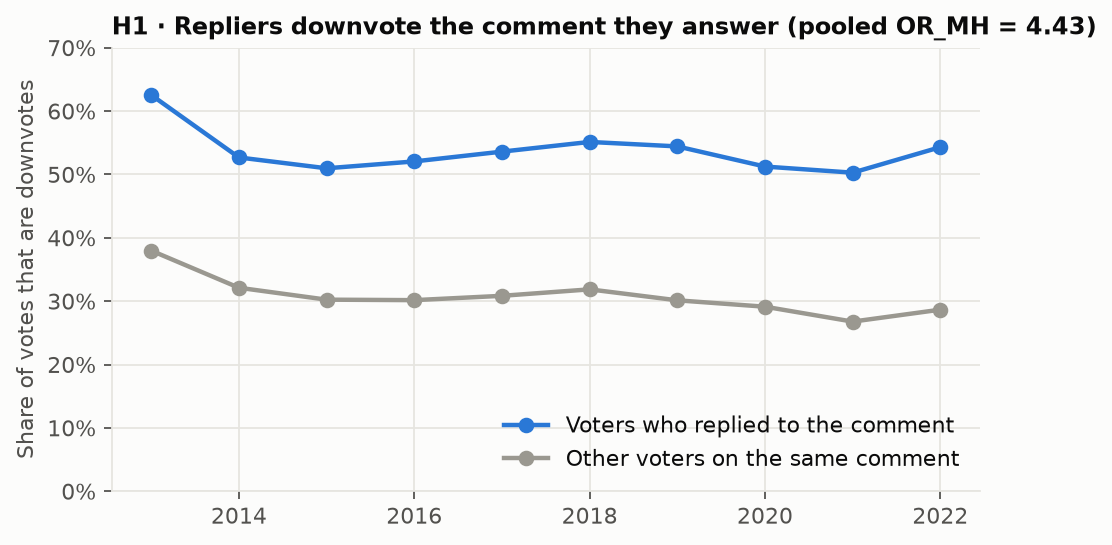
\includegraphics[width=0.85\textwidth]{04_h1_by_year.png}
\caption{H1 by year. Blue: share of downvotes among repliers' votes. Grey: among other voters on the same comments.}\label{fig:h1}
\end{figure}
\begin{readbox}
Each point is a year. The vertical gap between blue and grey is the effect in percentage points, about 20--25 points. Both lines move together (a downward step after 2013 and a slight rise afterwards), which means the \emph{overall mood} changes by year but the gap is stable. The shares are pooled shares; the title's 4.43 is the comment-stratified odds ratio, a different summary of the same pattern.\end{readbox}

\section{H2: the dyad analysis}
\begin{figure}[h]
\centering
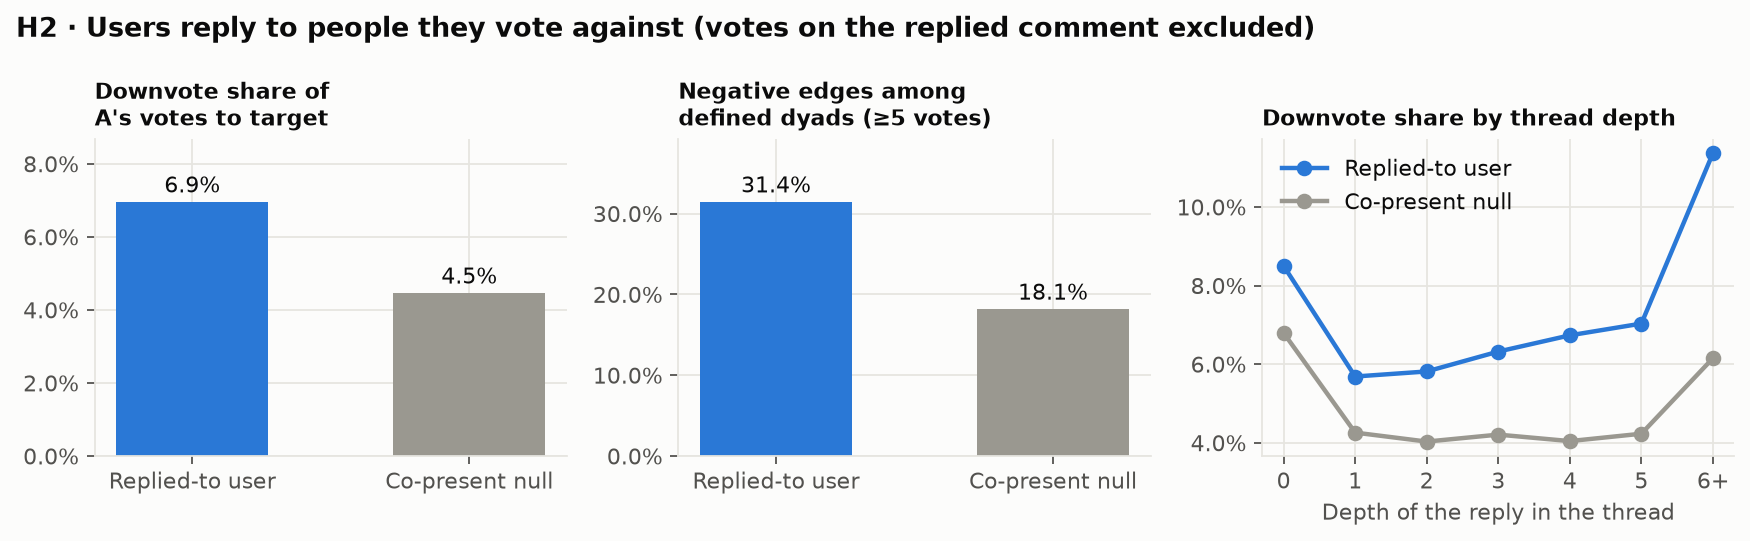
\includegraphics[width=\textwidth]{05_h2_dyad.png}
\caption{H2 with votes on the replied comment excluded. Left: $A$'s downvote share toward the target. Middle: share of negative edges among defined pairs. Right: downvote share by thread depth.}\label{fig:h2}
\end{figure}
\begin{readbox}
\textbf{Left:} 6.9\% against 4.5\% of $A$'s votes to the target are downvotes: low in absolute terms because most votes everywhere are upvotes, but 50\% higher in relative terms. \textbf{Middle:} the share of \emph{pairs} classified as negative: 31.4\% against 18.1\%. Remember that this panel uses only pairs with $\ge5$ votes (Section~\ref{sec:h2}). \textbf{Right:} the gap exists at every depth, and both lines rise for deeper replies (deeper conversations are more combative); the last point (6+) is pooled and based on fewer replies.
\end{readbox}

\section{Lifetime: CCDF and Kaplan--Meier}
\begin{figure}[h]
\centering
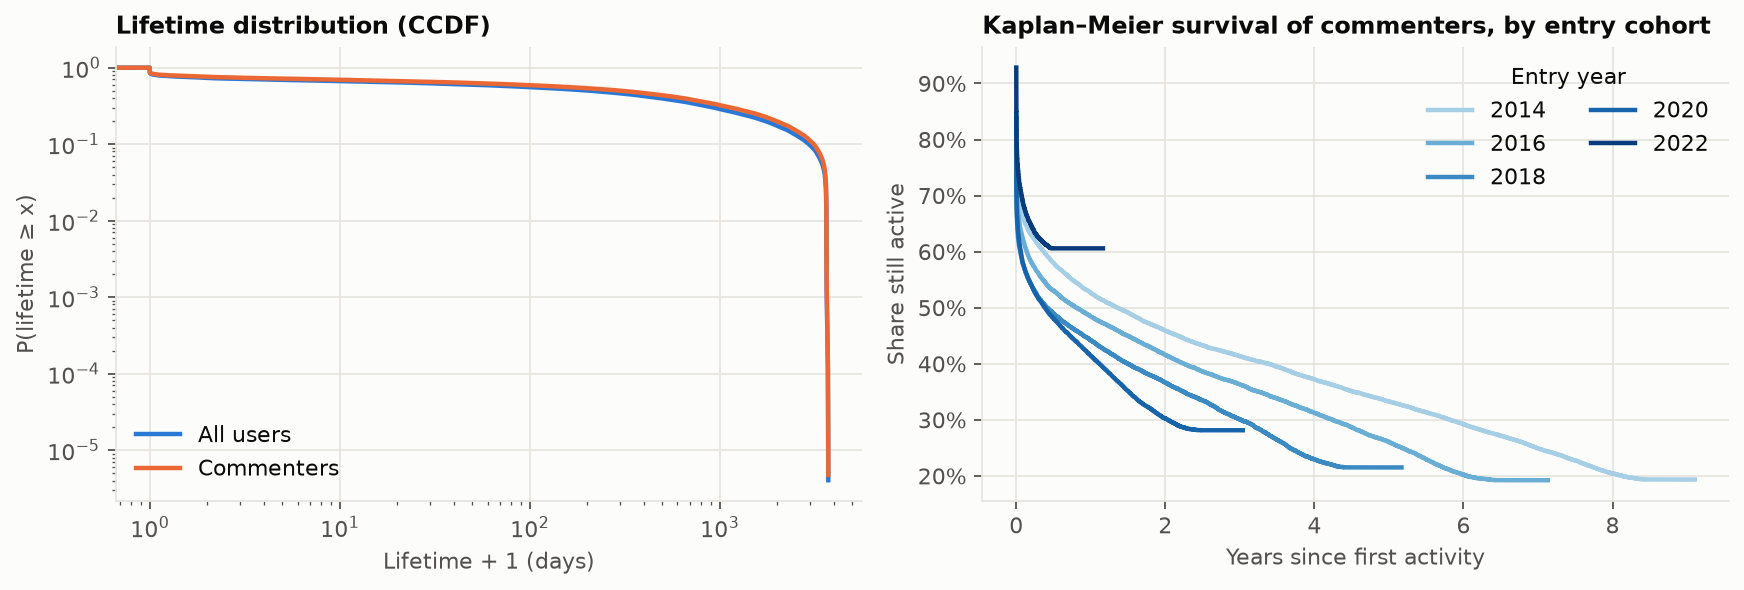
\includegraphics[width=\textwidth]{06_lifetime_ccdf_km.png}
\caption{Left: complementary cumulative distribution of lifetimes (log--log). Right: Kaplan--Meier survival by entry cohort.}\label{fig:km}
\end{figure}
\begin{readbox}
\textbf{Left:} a CCDF gives, for each $x$, the share of users with lifetime at least $x$; on log--log axes a straight line would mean a power law. Here the curve drops at 1 day (the 26.7\% one-day users), is nearly flat for a long time and falls sharply at about ten years, where the window ends. That final cliff is the window, not a behaviour. \textbf{Right:} each curve starts at 100\% and steps down when users leave. Steep initial drops are first-weeks churn. Curves end where the cohort's observation ends, and they \emph{flatten at the end} because the remaining users are censored and no longer counted as at risk. Later cohorts are lower: users who joined in 2018 or 2020 leave faster than those who joined in 2014. The 2022 cohort is short and mainly shows early churn.
\end{readbox}

\section{H4: the Cox model}
\begin{figure}[h]
\centering
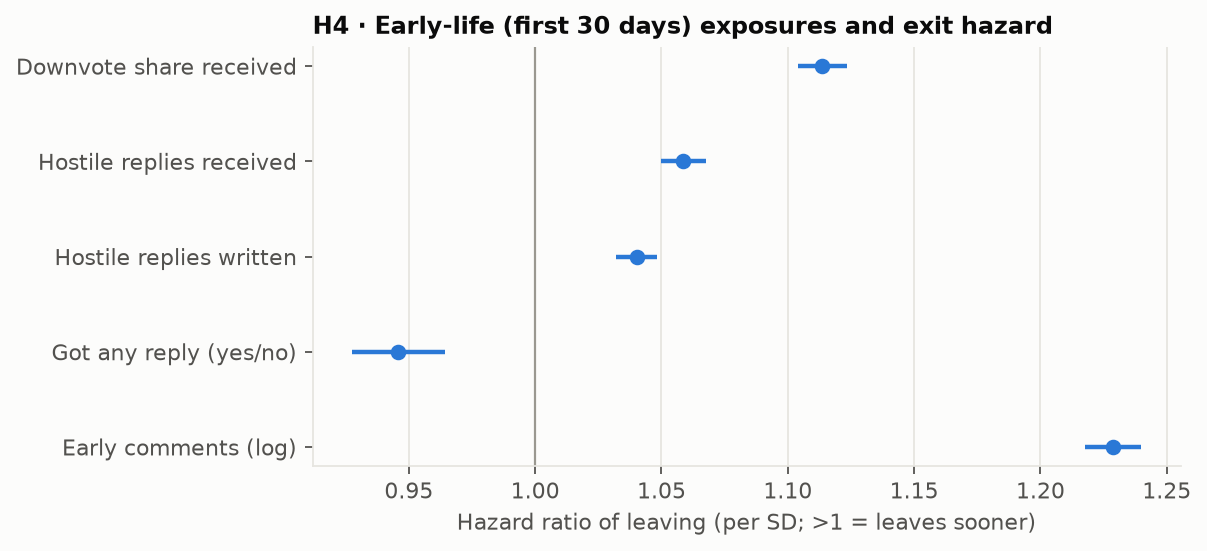
\includegraphics[width=0.9\textwidth]{06_h4_cox.png}
\caption{Hazard ratios of leaving per standard deviation of each early exposure; bars are 95\% intervals.}\label{fig:cox}
\end{figure}
\begin{readbox}
The vertical grey line is a ratio of 1 (no association). To the right of it, a higher value of the covariate goes with leaving sooner; to the left, later. Downvote share received (1.11) and hostile replies received (1.06) go with leaving sooner; getting any reply (0.95) with staying longer. The largest ratio is for the number of early comments (1.23), which is mostly an intensity signal. Intervals are narrow because of 98,670 users; their width does not tell you about bias.
\end{readbox}

\section{Multiverse}
\begin{figure}[h]
\centering
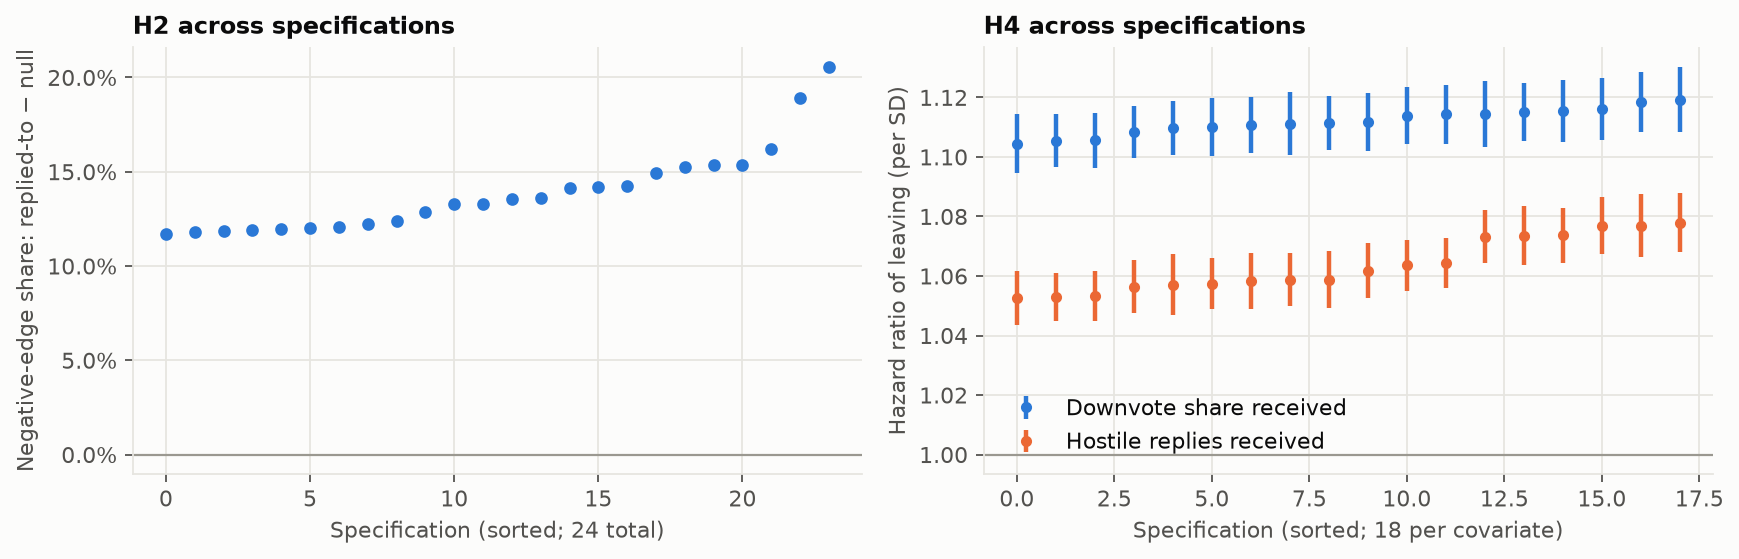
\includegraphics[width=\textwidth]{07_multiverse.png}
\caption{Left: H2 difference real $-$ null across 24 specifications, sorted. Right: H4 hazard ratios across 18 specifications.}\label{fig:multiverse}
\end{figure}
\begin{readbox}
Each dot is one analysis with a different combination of arbitrary choices. Dots are \emph{sorted by size}, so the x axis is an index, not a variable. What matters is whether any dot crosses zero (H2) or 1 (H4): none does. The spread of H2, 11.7 to 20.6 points, is an honest statement of how much the headline depends on the choices. The H4 ratios are tight because the specifications differ only in early window, churn buffer and shrinkage.
\end{readbox}

\section{Positive votes}
\begin{figure}[h]
\centering
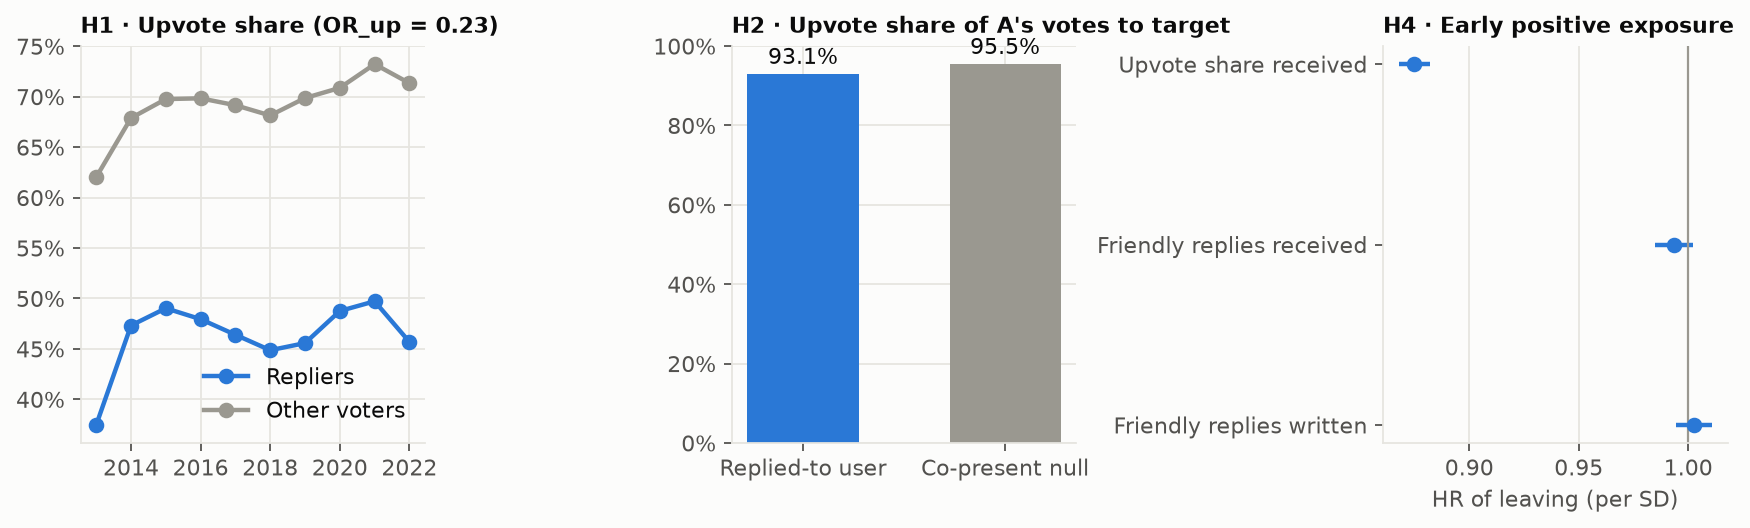
\includegraphics[width=\textwidth]{08_positive_votes.png}
\caption{Mirror of H1, H2 and H4 for positive votes.}\label{fig:pos}
\end{figure}
\begin{readbox}
Left: the mirror image of Figure~\ref{fig:h1} (repliers upvote less). The two figures contain the same information; do not count them as two findings. Middle: near ceilings (93\% against 95.5\%), so the same relative difference looks small. Right: only the upvote share received has a clear association with leaving (HR 0.87: more upvotes, later exit). Friendly replies are at 1.
\end{readbox}

\section{Long-lived users}
\begin{figure}[h]
\centering
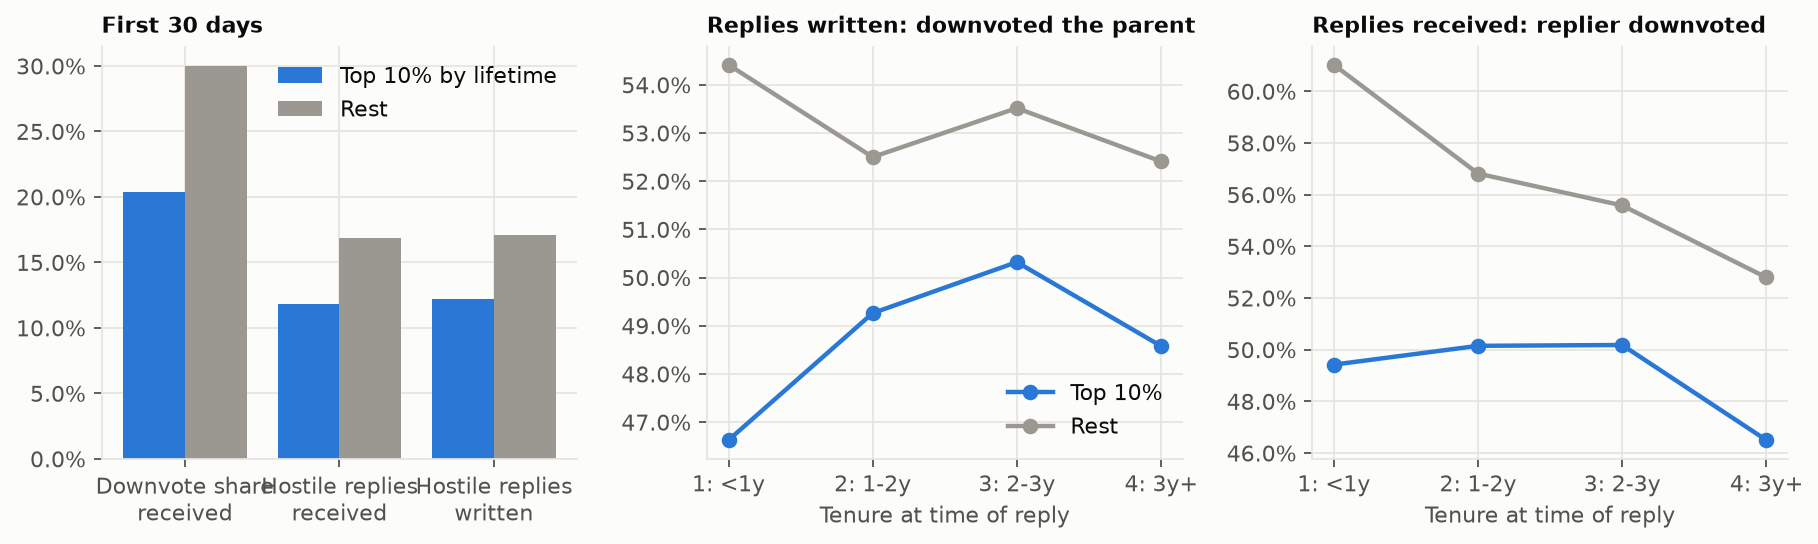
\includegraphics[width=\textwidth]{09_top_decile.png}
\caption{Top 10\% by lifetime within cohort versus the rest.}\label{fig:top}
\end{figure}
\begin{readbox}
Left: in the first 30 days the long-lived group receives fewer downvotes and fewer hostile replies, and writes fewer. Middle and right: by tenure at the time of the reply, the long-lived group less often downvotes the parent it answers (about 47--50\% against 52--54\% for the rest), and the replies it receives less often come from downvoters (46--50\% against 53--61\%). The curves of the rest fall with tenure on the right panel, the long-lived group's is flat. Read with Section~\ref{sec:longlived}: the group is mostly censored survivors.
\end{readbox}

\section{Which sentences the results do and do not allow}
\begin{tabularx}{\textwidth}{@{}Y Y@{}}
\toprule
Allowed & Not allowed \\
\midrule
``Users who reply to a comment downvote it more than other voters on that comment.'' & ``Replying is an act of opposition'' (no text; different voters) \\
``Real reply pairs are more often negative than co-present random pairs.'' & ``Users seek out opponents'' (article-level null is easy to beat) \\
``Early downvote exposure is associated with leaving sooner.'' & ``Downvotes cause users to leave'' (observational, untimed votes) \\
``The direction is stable across 24 and 18 specifications.'' & ``The effect is jointly significant across specifications'' (not tested) \\
``The long-lived group's first month looked less hostile.'' & ``Calm newcomers become long-lived'' (selected group) \\
\bottomrule
\end{tabularx}

\chapter{What is weak: a critical review}\label{ch:critique}

\begin{idea}
No coding error changes a headline number, but seven design points limit what the thesis may claim, and they are the ones a committee will find. Know them before it does.
\end{idea}

The full review is in \file{notes/experiments/01-reply-opposition-lifetime/CODE-REVIEW.md}. This chapter explains the findings in plain words, says what each fix would cost, and tells you what it would change.

\section{The three validity issues}

\subsection*{H-1: deleted users are invisible}
Users whose accounts were deleted do not appear as authors or voters. If banned or disgusted users delete their accounts, then \emph{the exits most related to hostility are exactly the ones we cannot see}. Direction of bias: probably toward \emph{underestimating} the association between hostility and leaving. Cost of a fix: none possible with this data. \emph{What to write:} state it as a limitation and restrict claims to users who keep an account.

\subsection*{H-2: the long-lived group is selected}
Explained in Section~\ref{sec:longlived}. Because lifetime ends at the last activity and the window ends in 2022, a large part of the ``top 10\%'' are people who are \emph{still there}. The group is ordered by when users were last seen, and early profiles are compared with a fixed threshold that mixes cohorts. \emph{Fix:} option B (a fixed ``survived $\ge3$ years'' among eligible cohorts) as the headline. Compute: about 5 minutes. Not run.

\subsection*{H-3: untimed votes in H4}
Votes have only a month. The ``first 30 days'' exposure may include votes cast up to a month later. This blurs the early window and slightly leaks later experience into the exposure. \emph{Fix:} none possible in the data; a sensitivity analysis could use only the comments (timed) to define exposure (hostile replies written and received, no votes).

\section{The six design issues}
\begin{description}
  \item[M-1 (H1).] Repliers and other voters are different people, and the interval treats comments as independent. A voter-level version (each voter as own control, with a bootstrap by voter) gives $3.49$ rather than $4.43$. \emph{Write:} report both, and say the first interval is too narrow.
  \item[M-2 (H2).] Defined-edge subsets differ between real and null pairs. \emph{Fix:} compare on pairs that are defined in \emph{both} or compare votes shares instead of edges.
  \item[M-3 (null).] Article-level null is easy to beat. \emph{Fix:} add a thread-level null (author of a random earlier comment in the \emph{same thread}), keeping both.
  \item[M-4 (depth).] The depth breakdown uses pooled shares, which mix compositions. \emph{Fix:} per-edge comparison within depth.
  \item[M-5 (hostility).] The ``hostile share'' (share of replies where the replier downvoted the parent) mixes how often someone votes with how hostile they are, since only replies where the replier \emph{voted} can be classified. \emph{Fix:} use the share among \emph{voted} replies.
  \item[M-6 (multiverse).] The multiverse is descriptive. Simonsohn's joint inference is not done; claims must say ``consistent across specifications''.
\end{description}

\section{Small items}
There are ten smaller items (L-1 to L-10), for example: how time zones are handled when assigning days; the proportional-hazards test was done on a 20,000-user sample; derived data are not versioned; inconsistent-timestamp comments are not excluded from lifetimes although the dataset authors recommend it (affecting under 0.15\% of users). They are listed in the review with proposed fixes. The ones that would rerun computation are on hold.

\section{New analyses designed but not run}
You decided today to wait. For the record, and so that you can pick them up in the order that is most useful:

\begin{longtable}{@{}p{4cm} p{7cm} p{2.4cm}@{}}
\toprule
Analysis & Question it answers & Compute \\
\midrule
\endhead
Period split (Lan Ceqin's periods: before 2020-W09; 2020-W09 to end 2021; from 2022-W01) & Does H1--H4 change before / during / after the 2020 COVID shift? Thread width and depth changed in those periods, so the pooled depth gradient mixes them. & minutes \\
Topic split (\texttt{Topic\_1}, top 8) & Is opposition concentrated in some topics? & minutes \\
Both directions of each pair & Is $A$'s stance toward $B$ mirrored by $B$'s toward $A$? & minutes \\
Activity strata (tertiles of comments) & Is the effect only a heavy-user effect? & minutes \\
Beta uncertainty propagation & How much do edge classifications change if the relation is itself uncertain? & about 10 min \\
Thread-level null & M-3 & about 10 min \\
Model-based null (popularity, recency, root bias, reciprocity, fitted per period) & A harder baseline than any uniform draw (Section~\ref{sec:null}) & fit on hundreds of threads per period; moderate coding \\
Factions against shuffled-sign and degree-preserving baselines & Do the two FAULTANA factions beat what random signed networks give? (Section~\ref{sec:h3}) & minutes, needs FAULTANA edges \\
Joint inference across specifications & Is H2 or H4 jointly significant over all specifications? (Section~\ref{sec:multiverse}) & tens of minutes \\
H4 with and without activity covariate; posts per day and burst measures & What do the vote-based covariates add beyond plain activity? (Section~\ref{sec:h4}) & minutes \\
Voter-level H1 with cluster bootstrap & M-1 & about 15 min \\
Equal-coverage H2, per-edge depth & M-2, M-4 & minutes \\
Redefined long-lived group & H-2 & about 5 min \\
Investigate the 2022 drop; burst accounts & Platform change, scripted accounts & exploratory \\
\bottomrule
\end{longtable}
Total about 35--50 minutes of compute for the original list; the four new rows add roughly an hour or two including coding. The bottleneck is not time, it is understanding what each result would mean, which is why this book comes first.

\section{A defence checklist}
\begin{enumerate}
  \item Why are votes a proxy for stance? What would a counterexample look like (sarcastic upvote, ``dislike'' as agreement with the wrong side)?
  \item Why compare with a co-present null rather than all users?
  \item Why is H1's 4.43 not the same as ``4.4 times as likely''?
  \item What does a hazard ratio of 1.11 mean, and what does it not?
  \item Which result would change if deleted users were visible?
  \item Why is the multiverse not a proof of robustness?
  \item Why is the long-lived group result not yet a conclusion?
  \item Why does H4 not contradict Cheng et al.\ 2014?
  \item Do your two factions beat a shuffled-sign baseline? (Honest answer today: not checked.)
  \item What does the hazard ratio of the vote-based covariates add beyond plain activity?
\end{enumerate}
Answers are in the text above; if one is hard, return to the section named in the answer.

\chapter{Sources: what to read, in what order, and why}\label{ch:sources}

\begin{idea}
About a dozen sources do real work in this thesis; read the first five carefully, the rest when you reach the method they support. Existence of each reference was checked online on 2026-11-02; the reusable per-paper summaries are in \file{notes/papers/PAPERS-SUMMARY.md}.
\end{idea}

\section{Priority order}
\begin{enumerate}
  \item \textbf{Fraxanet et al.\ (2026), the dataset paper.} (21 pages; 1 hour.) What each table is and what is inconsistent. Read the ``Internal consistency'' section twice.
  \item \textbf{Fraxanet et al.\ (2024), FAULTANA.} (12 pages and SI; 2 hours.) The source of the factions, the Beta prior and thresholds, antagonism and alignment.
  \item \textbf{Steegen et al.\ (2016)} (11 pages; 1 hour) and \textbf{Simonsohn et al.\ (2020)} (7 pages plus SI; 1.5 hours). Multiverse and specification curves.
  \item \textbf{Heider (1946)} (5 pages) and \textbf{Cartwright \& Harary (1956)} (17 pages). Balance theory in its original statement; 2 hours together; read the structure theorem in the second.
  \item \textbf{Lan Ceqin's thesis}, chapter~3 (periods and thread structure) and Appendix~A (generative thread models): the closest prior work on this dataset, and the source of the periods and the null-model idea.
  \item \textbf{Cheng et al.\ 2014}, for the discussion of H4.
  \item One survival text (\textbf{Kleinbaum \& Klein}, first chapters) and one categorical-data text (\textbf{Agresti}, chapters on $2\times2$ tables).
\end{enumerate}

\section{Local PDFs in the papers folder}
\begin{description}
  \item[Fraxanet et al.\ 2026, DerStandard dataset.] Table of sizes (586,942 articles; 75.6\,M comments; 412.5\,M votes; 247,863 users), field list, quality warnings (about 8\% deleted authors; vote counts replaced by aggregates from votes files; 1,208 comments with timestamps before their article, recommended to be excluded from lifetimes). Also states that factions are static.
  \item[Fraxanet et al.\ 2024 and SI, FAULTANA.] Method: find the two-group split that minimises frustrated edges; antagonism $\times$ alignment $=$ polarisation. DerStandard network: about 14.8\,k stable users, 5.56\,M edges, 41\% negative edges, 29\% frustrated edges, largest group 62\%. Edge rule: posterior mean outside $[0.4,0.6]$ and variance below $10^{-4}$. \emph{Caveat for H3:} factions use the same votes as our stance variables.
  \item[Lan Ceqin 2026, MSc thesis on reciprocity.] Weekly reciprocity networks; a jump in reply reciprocity around 2020-W09; same untimed-vote limitation; her period definitions are the proposed defaults for our period split. Our reply-back table is a signed, comment-level counterpart of her reciprocity.
  \item[Steegen et al.\ 2016.] Argues that a single analysis hides many arbitrary choices and proposes the multiverse. Section on how to display results.
  \item[Simonsohn et al.\ 2020 and SI.] Specification curves: define the set of reasonable specifications, plot the sorted estimates, and run a permutation-based joint test. We do only the first two steps.
  \item[Heider 1946; Cartwright \& Harary 1956.] Balance theory and its graph formalisation: a signed graph is balanced if and only if its nodes split into two groups with positive edges inside and negative between. Cartwright and Harary also warn that \emph{absence of a tie is not a negative tie}, which matters for ``no vote $\ne$ downvote''.
  \item[D'Ignazi et al.\ 2025; Amarasinghe et al.\ 2026.] Papers from the same group. D'Ignazi: ranking feedback loops amplify extremism (conceptual link only: extreme users engage more, which may confound hostility measures). Amarasinghe: decomposing uncertainty in prevalence estimates (an example of uncertainty accounting, not used here).
\end{description}

\section{Papers added on 2026-11-03 (downloaded, partly read)}
Fifteen further PDFs were downloaded from open sources into \file{notes/papers/}; each has an entry (D1--D15) in \file{PAPERS-SUMMARY.md} stating exactly how much was read. In order of usefulness for your thesis:
\begin{description}
  \item[Cheng et al.\ 2014, \emph{How community feedback shapes user behavior}.] The closest precedent for H4, and it \emph{appears to disagree} with it: negative feedback keeps people posting, while receiving \emph{no} feedback predicts leaving. Read it before writing the discussion of H4 (see D1 for how the two can be reconciled).
  \item[Cheng et al.\ 2015, \emph{Antisocial behavior in online discussion communities}.] Banned users, post deletion, and the warning that a downvote may mean disagreement rather than disapproval (a caveat for choice C1).
  \item[Wang et al.\ 2022, immortal-time review.] Landmark analysis and its cost: only users who survive to the landmark are analysed. Cite it next to Suissa 2008 for C12.
  \item[Leskovec et al.\ 2010 (two papers) and Easley \& Kleinberg ch.\ 5.] Signed edges, balance versus status theory, and \emph{weak} balance (several groups, not two). Important for the limits of the two-faction view in H3.
  \item[Danescu-Niculescu-Mizil et al.\ 2013.] User lifecycle and how they define abandonment (one year without posting; users near the end of the data are dropped), to compare with our censoring rule.
  \item[G\'omez et al.\ 2008 and 2013; Gonzalez-Bailon et al.\ 2010.] Supervisor-group work on reply networks and thread structure. The 2013 generative model (popularity, novelty, root bias) is the principled baseline for a stronger null model.
  \item[Kunegis et al.\ 2009; Aref \& Wilson 2018; Garimella et al.\ 2018; Kumar et al.\ 2018.] Related work on signed networks, balance measures, controversy and conflict; background only.
\end{description}
Not obtained: Hern\'an \& Robins (the Harvard server refused the download; get it from the authors' page) and Muchnik et al.\ 2013 (no free full text). The reading time for these is not included in the priority list above.


\textbf{Second reading pass.} The unread parts of Lan Ceqin's thesis (periods, generative thread models), the Simonsohn SI (joint inference), Cheng 2014 and 2015, Danescu-Niculescu-Mizil 2013, G\'omez 2013 and Leskovec 2010 were then read; their findings are entries E1--E7 of \file{PAPERS-SUMMARY.md}, and section F of that file lists six methodological implications (stronger null model, Lan Ceqin's periods, joint inference, H4 additions, a baseline check for the factions, and the caveat on votes). None has been implemented.

\section{Sources not on disk}
\begin{tabularx}{\textwidth}{@{}l Y l@{}}
\toprule
Topic & Source & Where it supports \\
\midrule
Signed networks & Leskovec, Huttenlocher \& Kleinberg (2010), \emph{Predicting positive and negative links in online social networks}, WWW & Chapter~\ref{ch:primer} \\
 & Easley \& Kleinberg (2010), \emph{Networks, Crowds, and Markets}, ch.~5 (free online) & Chapter~\ref{ch:primer} \\
Lifecycle and churn & Danescu-Niculescu-Mizil et al.\ (2013), \emph{No country for old members}, WWW, 307--318 & H4 \\
 & Cheng, Danescu-Niculescu-Mizil \& Leskovec (2015), \emph{Antisocial behavior in online discussion communities}, ICWSM & H4 \\
 & Kraut \& Resnick, \emph{Building Successful Online Communities} (MIT Press) & H4 \\
Threads & G\'omez, Kaltenbrunner \& L\'opez (2008), WWW, 645--654; G\'omez et al.\ (2013), \emph{World Wide Web} 16(5), 645--675 & replies; the supervisor's own work \\
MH and variance & Mantel \& Haenszel (1959), JNCI 22, 719--748; Robins, Breslow \& Greenland (1986), Biometrics 42, 311--323 & H1 \\
Bootstrap & Efron (1979), Annals of Statistics 7(1) (existence not verified in my search) & Section~\ref{sec:bootstrap} \\
Survival & Kaplan \& Meier (1958); Cox (1972), JRSS B 34, 187--220; Schoenfeld (1982) (not verified); Grambsch \& Therneau (1994), Biometrika 81, 515--526 & H4 \\
Immortal time / landmark & Suissa (2008), Am J Epidemiology 167, 492--499; Anderson, Cain \& Gelber (1983), J Clin Oncol 1, 710--719 & H4 \\
Bayes & Gelman et al., \emph{Bayesian Data Analysis} 3rd ed.\ (not verified) & H2, shrinkage \\
$p$-values and big data & Wasserstein \& Lazar (2016), Am Stat 70(2), 129--133; Lin, Lucas \& Shmueli (2013), ISR 24(4), 906--917 & C16 \\
Causal vocabulary & Hern\'an \& Robins, \emph{Causal Inference: What If} (free) & Chapter~\ref{ch:primer} \\
Tools & Raasveldt \& M\"uhleisen (2019), SIGMOD demo; Davidson-Pilon (2019), JOSS 4(40), 1317 & Chapter~\ref{ch:pipeline} \\
\bottomrule
\end{tabularx}

\begin{pitfall}
Citations marked ``not verified'' are standard references that my search did not locate. Check volume and pages before they enter the written thesis. Also, the supervisor's papers on reply behaviour (Andreas's group) are not in \file{notes/papers/}; ask for them.
\end{pitfall}

\section{Reading strategy}
Read every paper in three passes: (1) abstract, figures and conclusions (10 minutes) to decide whether it matters; (2) introduction and the section most relevant to your method; (3) only if you will cite or reuse it, the details. After each paper, write three lines in \file{notes/papers/}: what it claims, what you will borrow, what it cannot support in your thesis.

\chapter{Building on this work by yourself}\label{ch:building}

\begin{idea}
Every new analysis in this project follows one recipe: define the unit, build one row per unit with SQL, choose a comparison that removes the obvious confounder, attach an honest uncertainty, and write down what the result does \emph{not} show.
\end{idea}

\section{The recipe in six steps}
\begin{enumerate}
  \item \textbf{Question in one sentence.} ``Is $X$ different between group $G_1$ and group $G_0$?'' If you cannot write it, you are not ready to code.
  \item \textbf{Unit of analysis.} A comment, a pair, a user? The unit decides the SQL and which things are independent (and therefore what to resample).
  \item \textbf{Table of units.} One row per unit, written by a DuckDB query. Print 10 rows and check one by hand against the raw data.
  \item \textbf{Comparison.} Raw difference? Stratified (same comment, same article, same cohort)? Against a null? Name the confounder you are removing.
  \item \textbf{Uncertainty.} Resample the unit that is independent (user, comment). Report an interval, not a $p$-value.
  \item \textbf{Limits.} One paragraph in your notes: what could produce the same result without the effect you think you found?
\end{enumerate}

\section{Starting a new experiment}
\begin{lstlisting}
code/experiments/02-<short-name>/
    common.py        # copy from 01; change nothing but names
    01_<step>.py     # one question per script, with a docstring
notes/experiments/02-<short-name>/
    PLAN.md          # question, units, comparison, planned checks
    NOTES.md         # numbered decisions with [me]/[AI] tags
    RESULTS.md       # every number, with the script that made it
    results/
\end{lstlisting}
Write the \file{PLAN.md} \emph{before} the code, and list the checks you will run (for example, ``also by period, also by topic''). Writing the plan first makes the result honest: a check chosen after seeing the result is not a check.

\section{DuckDB patterns used here}
\begin{lstlisting}
-- 1. Always read Parquet directly; never load a 400M-row table into pandas
SELECT voter_id, count(*) FROM 'derived/votes_clean/*/*.parquet' GROUP BY 1;

-- 2. One 2x2 table per comment: conditional counts with FILTER
SELECT comment_id,
  count(*) FILTER (WHERE replied AND sign = -1) AS a,
  count(*) FILTER (WHERE replied AND sign =  1) AS b,
  count(*) FILTER (WHERE NOT replied AND sign = -1) AS c,
  count(*) FILTER (WHERE NOT replied AND sign =  1) AS d
FROM v GROUP BY 1;

-- 3. Keep only rows that have a match without duplicating columns
SELECT * FROM v SEMI JOIN (SELECT DISTINCT cid FROM repl) p ON v.comment_id = p.cid;
\end{lstlisting}
The script \file{h1\_voter\_strata.py} used in the review (stored in the session scratchpad, not in the repository) is a good small example of pattern 2. If you want it kept, copy it into \file{code/experiments/01-reply-opposition-lifetime/} with a number.

\section{Adding a robustness specification}
Open \file{07\_multiverse.py}. Specifications are built by a nested loop over a small grid (prior $\times$ thresholds $\times$ minimum votes $\times$ include/exclude). To add one dimension, add a list to the grid, add it to the loop and to the output table's columns. Rerun only \file{07}. The figure sorts specifications automatically.

\section{Checking a number you do not trust}
\begin{enumerate}
  \item Find the table in \file{results/} and the line in \file{run.log}.
  \item Recompute it from the Parquet files with a 10-line DuckDB query.
  \item Compute it on 100 rows by hand.
  \item If they differ, the SQL and not the statistics is the usual culprit: check join keys, filters, NULL handling.
\end{enumerate}

\section{Ideas that follow naturally (and how big they are)}
\begin{description}
  \item[Bridging users.] Who replies across the fault line, and are they treated differently? A separate experiment (your decision). It reuses factions (H3) and the reply-back table, plus a definition of ``bridge'' to be pre-registered.
  \item[Reply-choice model.] Fit the popularity--recency--root model of G\'omez et al.\ (2013), with Lan Ceqin's reciprocity extension, per period; use it as a null. Start from her sample design (size-stratified, about 684 threads per period).
  \item[Burst accounts and early prediction.] Add posts per day and the largest number of posts in one thread to the early features, and test how well the first 10 comments predict leaving, following Cheng et al.\ (2015).
  \item[Text.] With embeddings (not downloaded, 508\,GB) one could ask whether opposed replies are semantically distant. Out of reach for now; ask about cluster access.
  \item[Dynamics.] Does a user's stance change after being downvoted? Needs timed votes, which the data lack at fine resolution; month granularity may suffice.
  \item[Causality.] A natural-experiment angle: platform changes in 2022. Needs investigation of the drop first.
\end{description}

\section{Pre-specification, in plain words}
Before running a new analysis, write down in the plan: what you will compute, which outcomes, which subgroups, which thresholds and which checks. Afterwards, any additional analysis is labelled ``exploratory''. This protects you from fooling yourself, and it makes the multiverse chapter of the thesis easy to write. Three lines per analysis are enough.

\section{Writing the methods chapter}
For each analysis, answer: (1) the question; (2) the unit; (3) the exact estimator, with a citation; (4) how uncertainty is computed; (5) the choices that were not forced (pull them from the choice table in Section~\ref{sec:choices}); (6) a limitations sentence. If an answer takes more than a paragraph, split the analysis.

\section{Working habits that save time}
\begin{itemize}
  \item Commit after every working state; a first commit has not been made yet (all files are untracked). A commit message that says what changed and why is documentation.
  \item Never edit derived Parquet files by hand.
  \item Keep AI use labelled: every decision tagged [me], [AI, reviewed] or [AI, not yet reviewed]. Move items to ``reviewed'' only when you could explain them from understanding (\file{notes/method/AI-USE.md}).
  \item When something surprises you, put it in \file{PREGUNTAS.md}; surprises are the raw material for the discussion section.
\end{itemize}


\appendix
\chapter{Glossary and frequently asked questions}\label{app:glossary}

\section*{Glossary}
\begin{description}
  \item[Antagonism] share of interactions that are negative (FAULTANA).
  \item[Alignment] how well negative interactions follow the two-camp split (FAULTANA).
  \item[Beta distribution] distribution over a probability between 0 and 1; the Beta$(\alpha,\beta)$ prior updated by counts gives the posterior used for pair relations.
  \item[Bootstrap] resampling to estimate uncertainty (Section~\ref{sec:bootstrap}).
  \item[Censoring] the event of interest (leaving) is not observed within the window; right-censored: still active at the end; left-censored: began before the window.
  \item[CCDF] complementary cumulative distribution function, $P(X\ge x)$.
  \item[Balance, weak balance] a signed network is balanced if every triangle has three positive edges or one positive and two negative; it then splits into two camps. Weak balance also allows triangles with three negative edges and then several camps.
  \item[Frustration index] the least number of edges whose removal (or sign flip) makes a signed network balanced; hard to compute exactly.
  \item[Joint inference] a single test of whether the effect is zero in all specifications of a multiverse, by resampling under the null.
  \item[Popularity, novelty, root bias] the three ingredients of the thread-growth model of G\'omez et al.\ (2013).
  \item[Status theory] a positive link means the source regards the target as higher in a ranking; it explains directed signed links better than balance (Leskovec et al.\ 2010).
  \item[Cohort] group of users who first appeared in the same year.
  \item[Co-present null] random alternative target: author of a random earlier comment in the same article.
  \item[Confounder] a variable that affects both the exposure and the outcome and so distorts their comparison.
  \item[Cox model] regression for hazards; coefficients are log hazard ratios.
  \item[Dyad] an ordered pair of users $(A,B)$.
  \item[Edge] a reply from $A$ to $B$ (reply network) or a signed relation (stance network).
  \item[Faction] one of the two camps from FAULTANA.
  \item[Frustrated edge] an edge that violates balance: negative inside a camp or positive between camps.
  \item[Hazard ratio] ratio of instantaneous rates of leaving between two covariate values.
  \item[Immortal-time bias] bias from counting time during which the event could not have happened.
  \item[Kaplan--Meier] nonparametric survival estimate that handles censoring.
  \item[Landmark] a fixed time (day 30) from which follow-up starts, using only users still at risk.
  \item[Mantel--Haenszel] pooled odds ratio across strata.
  \item[Multiverse] the set of defensible analyses under alternative arbitrary choices.
  \item[Null model] a baseline that preserves some structure and randomises the thing being tested.
  \item[Odds ratio] ratio of odds; 1 means no difference.
  \item[Parquet] a compressed columnar file format.
  \item[Proxy] an observable variable standing in for an unobservable one (votes for stance).
  \item[Shrinkage] pulling a noisy estimate toward a population value.
  \item[Specification curve] plot of estimates across specifications, sorted by size.
  \item[Stratum] a subgroup within which a comparison is made.
  \item[Thread] a top-level comment and all the replies under it.
\end{description}

\section*{Frequently asked questions}
\begin{description}
  \item[Why not just use text?] The released data have none. Embeddings exist but are very large; the project works with votes.
  \item[Is a downvote really opposition?] Often, but not always: people downvote rudeness, off-topic or errors without disagreeing with the position. Treat votes as a signal of \emph{disapproval of the comment}; stance is an interpretation. The thesis should say so in its limitations.
  \item[Why 53\% vs 30\% but OR 4.43?] The odds ratio is computed within each comment and then pooled; the pooled shares are a coarser summary. See Section~\ref{sec:h1}.
  \item[Why is H1 the same as its positive-vote mirror?] Because for one table the two odds ratios are reciprocals.
  \item[Why 200 bootstrap replicates?] A balance of cost and stability for an interval; 1,000 would shift the endpoints very little.
  \item[Why landmark at 30 days?] A trade-off: later gives more exposure but removes more users; the multiverse tries 14 and 60 days.
  \item[Does HR 1.11 mean 11\% more users leave?] No: the rate of leaving is 11\% higher at any moment per SD of exposure.
  \item[Can I say that downvotes cause exit?] No. Observational, untimed votes, selected users.
  \item[What is the first thing to do before rerunning everything?] Commit the current state, so differences can be examined afterwards.
\end{description}

\chapter{Exercises with answers}\label{app:exercises}

Do them on paper first. Python is allowed for the last ones.

\begin{enumerate}
  \item Compute the odds and the OR for downvote shares 20\% and 10\%, then for 2\% and 1\%. What happens to the OR relative to the risk ratio?
  \item In Section~\ref{sec:h1}'s toy, change table Y to $(2,8,8,32)$ so its inside OR is 1.0 still, then to $(4,6,8,32)$. Predict whether MH goes up or down in each case and check with \file{mh\_toy.py}.
  \item With prior Beta$(1,2)$, a pair has 3 positive and 12 negative votes. Compute $E[p]$ and the edge sign. Then with 3 positive and 4 negative votes.
  \item A user has 2 replies, 1 hostile. The population share is 0.20 and $M=2$. What is the shrunk share? What if they had 20 replies, 10 hostile?
  \item KM: users leave at years 1, 3, 3 and are censored at 2 and 5. Compute $S(t)$ at each leaving time.
  \item Explain in two sentences why H1's interval is too narrow.
  \item Explain why the share of negative edges in H2 is not directly comparable between real and null pairs.
  \item A hazard ratio is 0.95 for ``got any reply''. State it in a sentence that a non-statistician understands.
  \item Why must the landmark Cox model exclude users who left before day 30?
  \item Name two ways the long-lived group can look ``calmer'' without calm users being more likely to stay.
\end{enumerate}

\section*{Answers}
\begin{enumerate}
  \item 20\%: odds 0.25; 10\%: 0.111; OR $=2.25$, risk ratio 2. 2\%: 0.0204; 1\%: 0.0101; OR $=2.02$, risk ratio 2. The OR approaches the risk ratio as the event gets rare, and exaggerates it when the event is common.
  \item $Y=(2,8,8,32)$ has inside OR $2\cdot32/(8\cdot8)=1$, like the original Y, but the downvote shares are higher, so Y's weight changes and MH falls from 1.58 to 1.44. $Y=(4,6,8,32)$ has inside OR $4\cdot32/(6\cdot8)=2.67$, above X's 2, so MH rises to 2.33. (Values computed with \file{mh\_toy.py}.)
  \item $3$ positive, $12$ negative: $E[p]=(3+1)/(15+3)=0.222$, negative. $3$ positive, $4$ negative: $E[p]=(3+1)/(7+3)=0.40$; not below 0.4, so no edge (and the pair has 7 votes, enough for the $\ge5$ rule).
  \item $(1+2\cdot0.2)/(2+2)=0.35$. With 10 of 20: $(10+0.4)/(22)=0.473$.
  \item At $t=1$: 5 at risk, 1 leaves, $S=0.8$. At $t=3$: users at risk are those with time $\ge3$: the two leaving at 3 and the one censored at 5, so 3 at risk, 2 leave, $S=0.8\cdot(1-2/3)=0.267$. The user censored at 2 left the risk set before $t=3$ without being counted as leaving.
  \item Many votes on different comments come from the same voters, and the interval treats comments as independent, so the effective sample size is overstated. The voter-level analysis gives a smaller effect with wider uncertainty.
  \item Real pairs more often reach five votes (repliers have a history with the people they answer), so the two shares come from different sets of pairs; a compositional difference could drive part of the gap.
  \item ``Among users who are still active at day 30, those who received a reply in their first month left at a slightly lower rate than those who did not (5\% lower, after accounting for cohort and other early exposures).''
  \item Because exposures are measured in the first 30 days; a user who left earlier would have an incomplete measurement, and including them would credit the exposure with time they could not have left.
  \item (a) The group is composed of survivors from earlier cohorts, which differ in tone; (b) quiet users who vote little receive few downvotes and also keep a long, low-intensity presence; (c) the share measures the \emph{rate} of downvotes which depends on how often the user writes controversial things, not on being calm.
\end{enumerate}

\chapter{File map and reproduction}\label{app:filemap}

\section*{Repository map}
\begin{longtable}{@{}p{5.8cm} p{8cm}@{}}
\toprule
Path & What is there \\
\midrule
\endhead
\file{INDEX.md} & start page of the vault \\
\file{code/pyproject.toml}, \file{uv.lock} & Python environment \\
\file{code/experiments/01-reply-opposition-lifetime/} & scripts 00--09, \file{common.py}, \file{h4.py}, \file{plotstyle.py}, checks \\
\file{data/derstandard/} & raw tables and \file{derived/} Parquet (not versioned) \\
\file{notes/dataset/} & README, codebook, data-treatment notes \\
\file{notes/experiments/01-reply-opposition-lifetime/} & plan, notes, results, explanations, code review, \file{results/} \\
\file{notes/papers/} & PDFs and \file{PAPERS-SUMMARY.md} \\
\file{notes/meetings/} & meeting notes (2026-09-30, 2026-10-19) \\
\file{notes/method/AI-USE.md} & how AI is used and labelled \\
\file{notes/guide/} & this book, plus the two earlier guides \\
\bottomrule
\end{longtable}

\section*{Rebuilding this book}
\begin{lstlisting}
cd notes/guide/book
pdflatex main.tex
pdflatex main.tex     # second pass for the table of contents and references
\end{lstlisting}
The figures are read from the experiment's \file{results/} folder (see \texttt{graphicspath} in \file{main.tex}); regenerate them by rerunning the scripts and the book picks them up. Snippets in \file{snippets/} are the sources of the code listings; run them with \texttt{python snippets/mh\_toy.py}.

\section*{Where the numbers in this book come from}
\begin{tabularx}{\textwidth}{@{}l Y@{}}
\toprule
Number & Source \\
\midrule
Funnel (53,427,803 $\to$ 44,350,672) & \file{results/01\_reply\_funnel.csv} \\
H1 (4.43; 53.3 vs 30.1\%) & \file{results/04\_h1\_comment\_level.csv} \\
H2, H3, reply-back & \file{results/05\_*.csv} \\
Lifetime, KM, Cox & \file{results/06\_*.csv} \\
Multiverse ranges & \file{results/07\_multiverse\_h2.csv}, \file{07\_multiverse\_h4.csv} \\
Positive votes & \file{results/08\_*.csv} \\
Long-lived users & \file{results/09\_*.csv} \\
Voter-stratified H1 (3.49) & diagnostic in session scratchpad (\file{h1\_voter\_strata.py}); documented in \file{CODE-REVIEW.md} \\
\bottomrule
\end{tabularx}


\end{document}
